\chapter{Computer Science}
\label{chapter:computer-science}

\section{Solution Design}
\label{chapter:design}

This section aimed to fully describe the solution design from a top to bottom approach. First of all, the general idea of the design was described, abstracting every detail to easily understand the whole. Later on, the different sections of the design were explained with all their characteristics described. The implementation details were left for the following sections, whereas here we only focused on the ideas and methods used.

In short, the solution to the problem of studying what an observer near a black hole would see is a ray tracer, that is, a device that computes the origin of the rays of light that arrives to a virtual camera placed in a virtual universe.

This work implemented a general relativity ray tracer; \ie, a ray tracer for which the path followed by light is not always a straight line.

In \autoref{sec:gendesc}, the layout of the solution is depicted, whereas in \autoref{sec:parallel}, the parallelization designed is explained. \autoref{sec:pinhole} explains the pinhole camera model, describing the identification of each pixel on the camera with a lightlike particle coming from the celestial sphere. Finally, \autoref{sec:initcond} and \autoref{sec:numerical} describes the necessary work to numerically solve the geodesic equations.

\subsection{General Description}
\label{sec:gendesc}

Imagine a spacetime defined by a Kerr metric, with a black hole on its centre, and a camera with a digital sensor placed near it.

As we have had studied, all rays that hit the sensor followed a geodesic to finally arrive to the camera, and their paths were of great interest for us: the origin of the ray told us what the particular pixels saw and the curvature of the geodesic let us understand the geometric nature of the spacetime.

For every pixel on the sensor, the ray tracer work was abstracted as a function that computed the path of the ray that hit it. Therefore, from the pixel coordinates, $p = (p_x, p_y)$, it computed the geodesic path followed by the ray.

This point was computed using the \ac{ODE} system described in \autoref{theo:eqsmotion}, derived from the Kerr spacetime. Therefore, a numerical solver for such systems was needed, along with the initial conditions of each ray. This conformed an \ac{IVP}, a well-known problem whose numerical solutions were widely studied.

Abstracting all these tasks out, the general outline of the ray tracer was described on \autoref{alg:raytracer}.

\begin{algorithm}
	\caption{High-level abstraction of the ray tracer}
	\label{alg:raytracer}
	\begin{algorithmic}[1]
		\Function{Ray Tracer}{}
		\State ODEsystem $\gets$ Geodesics equations for the Kerr spacetime
		\State Camera $\gets$ Pinhole camera model
		\State Geodesics $\gets \{\emptyset\}$
		\For{pixel $p = (p_x, p_y)$ in the Camera sensor}
		\State initCond $\gets$ initConditions($p_x$, $p_y$)
		\State $\gamma_{xy} \gets$ solveInitValueProblem(ODEsystem, initCond)
		\State Geodesics $\gets$ Geodesics $\cup$ $\gamma_{xy}$
		\EndFor
		\Return{Geodesics}
		\EndFunction
	\end{algorithmic}
\end{algorithm}

The solution designed for the ray tracer was based on the algorithm described in \cite{thorne15}, which assumes the following:
\begin{enumerate}
	\item The spacetime is defined by the Kerr metric written in \ac{BL} coordinates with a black hole in the centre, parametrized by its spin $a$, with mass 1.
	\item The \ac{FIDO} is a locally non-rotating observer. We define a family of \acp{FIDO} at rest in space with orthonormal basis vectors $\{e_r, e_\vartheta, e_\varphi\}$, pointing along the spatial coordinate lines.
	\item A camera is placed outside of the horizon of the black hole, whose position is described by the coordinates $\{r_c, \vartheta_c, \varphi_c\}$, its speed with respect to the \ac{FIDO} is noted as $\beta$, its direction of motion relative to the \ac{FIDO} is described by a unit vector $B$ in the camera's reference frame and there is a right-handed coordinate system placed on the camera's reference frame, with the orthonormal basis $\{e_x, e_y, e_z\}$, where
		\begin{itemize}
			\item $e_y$ is identified with $B$.
			\item $e_x$ is perpendicular to $e_y$ and contained on the plane $\langle e_{\widehat{r}}, e_{\widehat{\vartheta}} \rangle$.
			\item $e_z$ is perpendicular to $e_x$ and to $e_y$.
		\end{itemize}
		We also set up a spherical coordinate system derived from the previous one, noted as $\{\vartheta_{cs}, \varphi_{cs}\}$, where $\vartheta$ is the polar angle with respect to the coordinate system origin and $\varphi$ is the azimuthal angle with respect to the coordinate system origin. The black hole is assumed to rotate in the positive $\varphi$ direction.
\end{enumerate}

The algorithm considered a set of timelike geodesics arriving at the camera. These geodesics were then integrated backwards to obtain the ray's point of origin on the celestial sphere (at $r = \infty$). These points were noted as $(\vartheta', \varphi')$.

In short, the algorithm goal was to compute the following map
\begin{equation}
\label{eq:initmap}
(\vartheta_{cs}, \varphi_{cs}) \xmapsto{\mathfrak{h}_1} (\vartheta', \varphi')
\end{equation}
for each considered geodesic arriving at the camera.

\subsection{Parallelization Techniques}
\label{sec:parallel}

A ray tracer is in general highly parallelizable, and our design was not different: it performed the exact same operation on a large set of different data; namely it solved the \ac{ODE} system, whose equations (\autoref{theo:eqsmotion}) were always the same, on a large number of different initial conditions.

The idea behind the parallelization design was easy: for each parallelized node, we have to feed the numerical solver with a different initial condition, compute from each pixel of the image. Using the classic Flynn's taxonomy \cite{flynn72} terminology, our architecture followed a \ac{SIMD} paradigm, where a single generalized task works on multiple data streams in order to compute multiple results.

Ideally, we would have liked to design a completely parallel solution, in which we had the same number of nodes in the parallel architecture as pixels we had in the image. Although this was highly difficult for large images with the classic parallelization on \acp{CPU}, the new \ac{GPU} techniques helped us get closer to this goal.

\subsubsection*{General-Purpose Computing on Graphics Processing Units}

Historically, \acp{GPU} have been used to process tasks and data always related to computer graphic purposes, whereas \acp{CPU} have been used in general computation.

In recent years, a new powerful technique has been deeply studied: the so-called \ac{GPGPU}. Its goal is to use the \acp{GPU}, designed to have thousands of cores that can process data in parallel, to general purpose computing, not only computer graphics tasks.

Although each of the cores on a \ac{GPU} is much less powerful than a single \ac{CPU}, the great order of parallelization ---thousands of cores in a \ac{GPU} against just a few dozens of them on \acp{CPU}--- and the specific design to handle a parallel architecture makes the use of \ac{GPGPU} appealing when one wants to design an efficient solution.

Our ray tracer used this paradigm, virtually parallelizing the computation of each geodesic in a different \ac{GPU} core. We say \emph{virtually} because the number of cores in a \ac{GPU} is always finite, and for large images, some computations were serialized. However, as we saw later, this was transparent to us, developers, by using a proper \ac{GPGPU} library.

\subsubsection*{Parallelized Solution}

With this paradigm in mind, we described the parallelized solution by modifying the main loop on \autoref{alg:raytracer}, whose iterations were split across all the nodes on the \ac{GPU}.

If we abstract the computation of the geodesic that hits one single pixel in a function, as shown in \autoref{alg:onepixel}, we were able to finally define the layout of the parallelized solution.

\begin{algorithm}[bth]
	\caption{Single pixel geodesic computation}
	\label{alg:onepixel}
	\begin{algorithmic}[1]
		\Function{ComputeGeodesic}{$p_x, p_y$, Geodesics}
		\State initCond $\gets$ initConditions($p_x$, $p_y$)
		\State $\gamma_{xy} \gets$ solveInitValueProblem(ODEsystem, initCond)
		\State Geodesics $\gets$ Geodesics $\cup \gamma_{xy}$
		\EndFunction
	\end{algorithmic}
\end{algorithm}

\autoref{alg:raytracer2} shows the parallelized solution following the \ac{SIMD} paradigm. The solution was similar to the one shown at \autoref{alg:raytracer} but with a little change: the loop was parallelized and each pixel was computed at a different node of the parallel architecture.

\begin{algorithm}
	\caption{High-level abstraction of the ray tracer}
	\label{alg:raytracer2}
	\begin{algorithmic}[1]
		\Function{Ray Tracer}{d}
		\State ODEsystem $\gets$ Geodesics equations for the Kerr spacetime
		\State Camera $\gets$ Pinhole camera model
		\State Geodesics $\gets \{\emptyset\}$
		\State $(\textrm{Node}_1, \dots, \textrm{Node}_n) \gets$ Initialize parallel device
		\For{pixel $p^i = (p^i_x, p^i_y)$ in the Camera sensor}
		\State ComputeGeodesic($p^i_x, p^i_y$, Geodesics) at $\textrm{Node}_i$
		\EndFor
		\Return{Geodesics}
		\EndFunction
	\end{algorithmic}
\end{algorithm}

\subsection{Pinhole Camera}
\label{sec:pinhole}

The camera was abstracted as a simple, yet effective, model that let us produce realistic images of what an observer would see when looking at a black hole from near distances. It followed the \emph{pinhole camera model}, which assumes a camera with an infinitely small diaphragm that focuses all the incoming rays onto its sensor.

The camera was described by the following parameters: the position on the Kerr spacetime, described by the spatial \ac{BL} coordinates $\{r_c, \vartheta_c, \varphi_c\}$;the \emph{sensor} (that can be thought as the film or the CCD of a usual camera), which is described by its \emph{resolution} (number of pixels per column and number of pixels per row) and by its size (width and height in physical units); the \emph{focal point}, $F$: a point in the line perpendicular to the sensor and going through its centre ---this point collected all incoming rays and can be though as the diaphragm, whose aperture is infinitely small---; the \emph{focal distance}, $d$: distance from the focal point to the sensor; the \emph{pitch}, \emph{roll} and \emph{yaw} angles, that describe the rotation of the sensor on each of its axis.

This model let us compute the direction of the incoming rays just by indexing the particular pixel they hit, obtaining a map $(p_x, p_y) \xmapsto{\mathfrak{h}_2} (\vartheta_{cs}, \varphi_{cs})$, where $(p_x, p_y)$ are the components of the pixel in a system of coordinates whose origin is placed at the top-left corner of the sensor.

By composing \autoref{eq:initmap} and previous map, we defined the map $(p_x, p_y) \xmapsto{\mathfrak{h} = \mathfrak{h_1}\circ\mathfrak{h_2}} (\vartheta', \varphi')$, that summarises all the work the algorithm does: from a pixel on the camera's reference frame, we computed the origin of the incoming ray that hit that pixel.

\subsubsection*{Pixel to Ray Map}
\label{subcsec:pixeltoray}

Let us consider a pixel $P$ whose coordinates on the sensor's reference frame are, in physical units, $(p_x, p_y)$, as depicted in \autoref{fig:pinhole}.

\begin{figure}[bth]
	\myfloatalign
	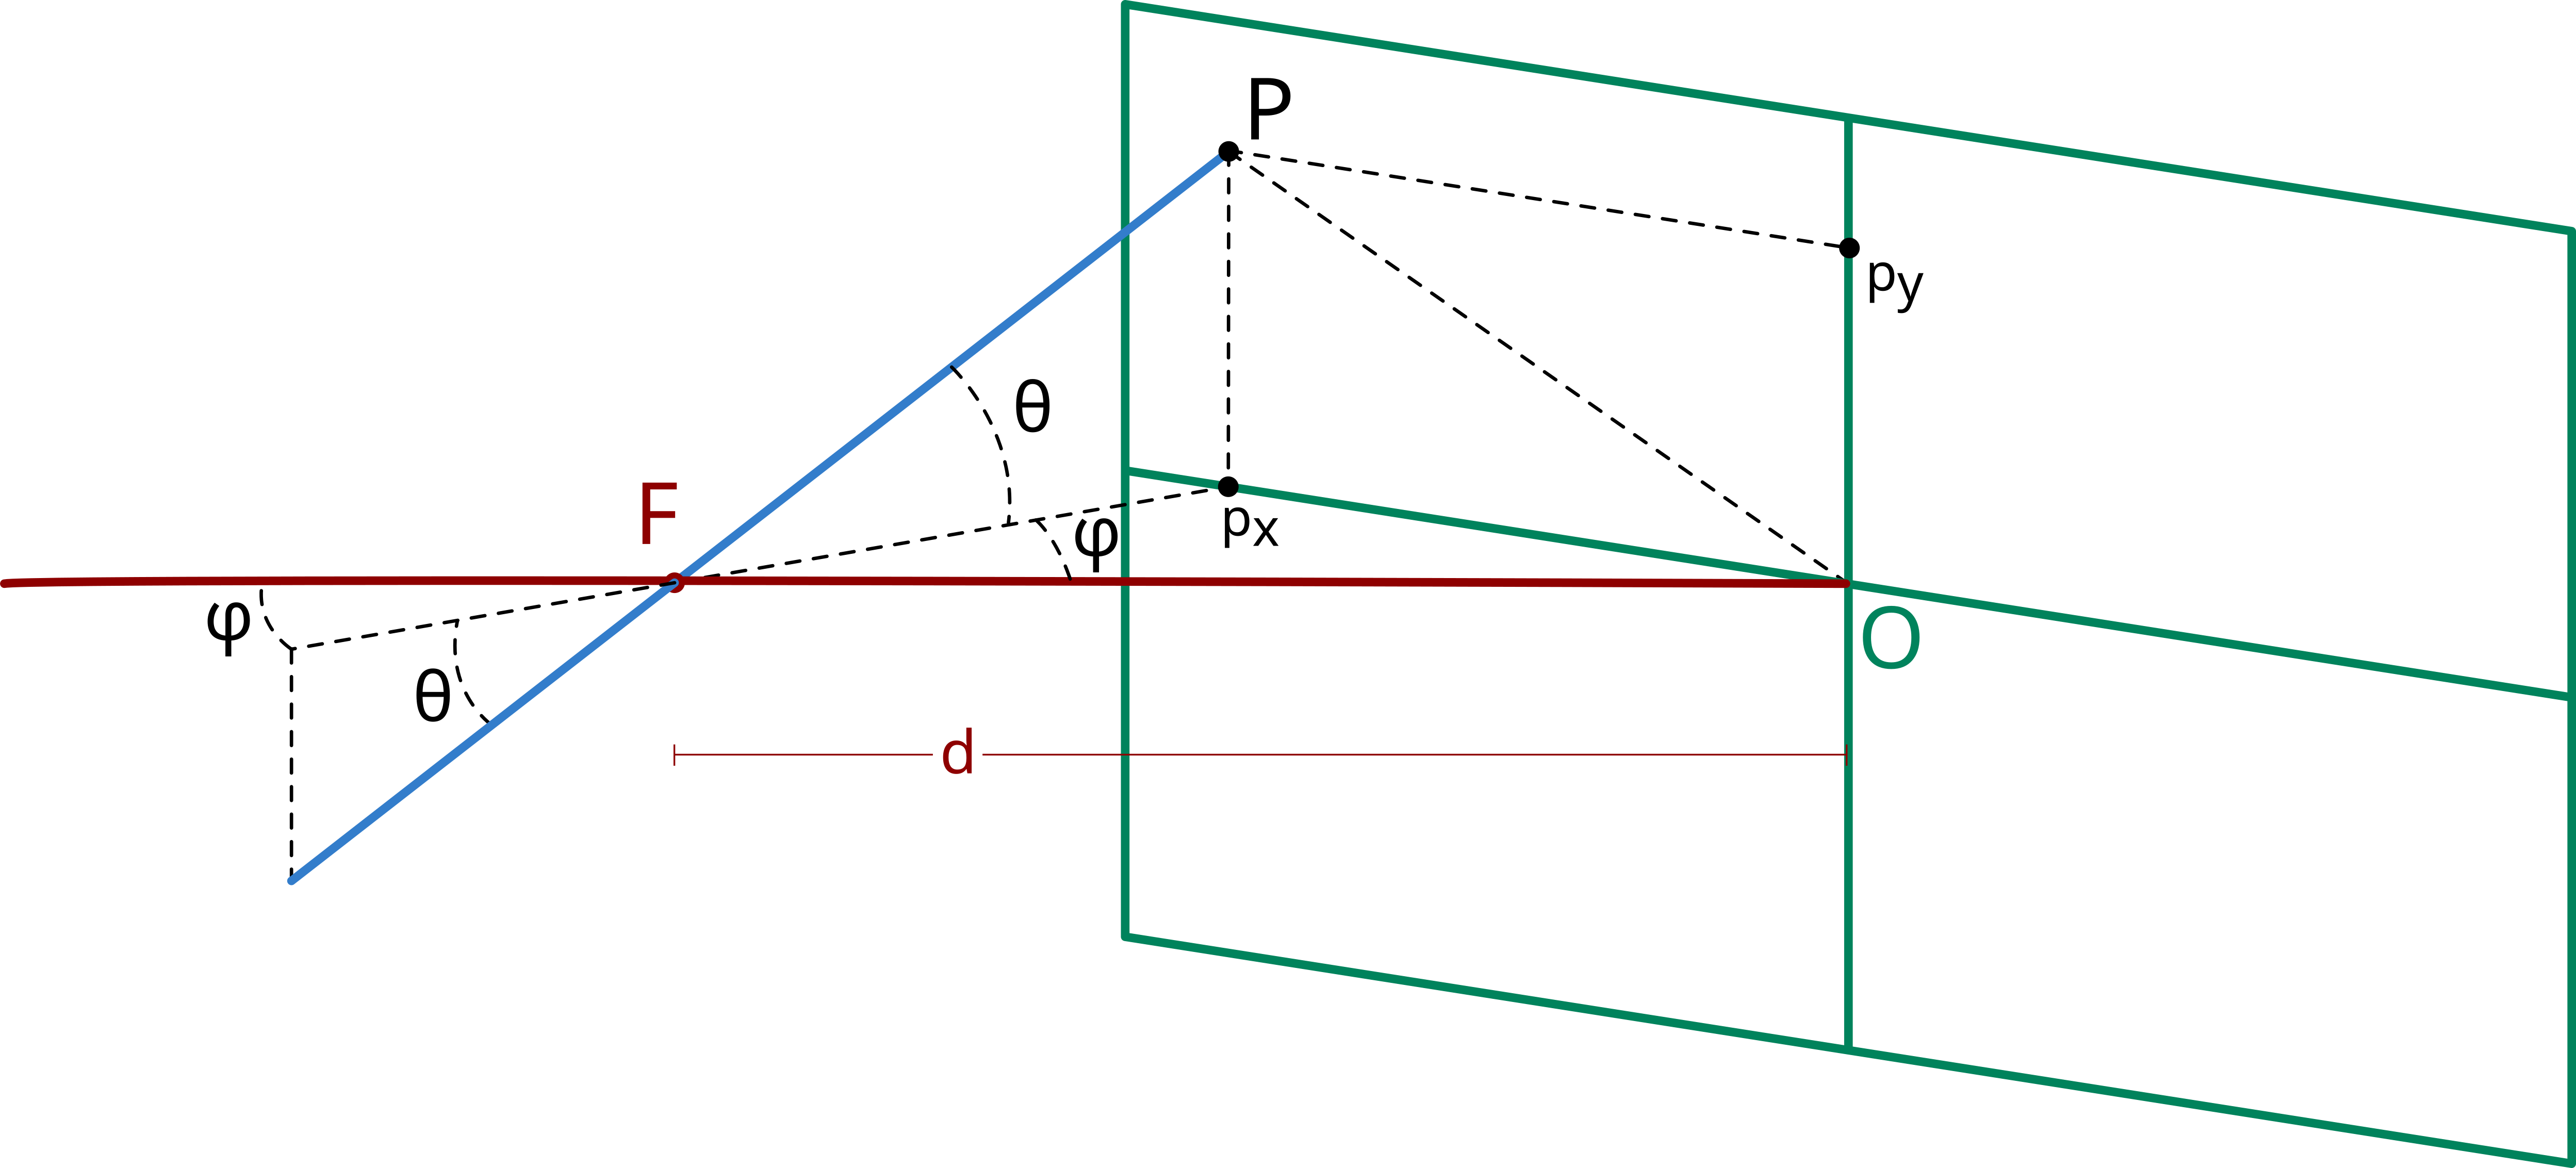
\includegraphics[width=.7\linewidth]{gfx/pinhole.png}
	\caption[Pinhole camera model]{Pinhole camera model}
	\label{fig:pinhole}
\end{figure}

All rays that hit the sensor were assumed, by our model, to pass through the focal point $F$. Thus, we computed the angles $\vartheta$ and $\varphi$ for the ray hitting the sensor at pixel $P$ with elementary trigonometry. This is detailed in the original work, and as a result we got the equations
\begin{equation}
\label{eq:pinhole1}
\vartheta_{cs} = \eta + \frac{\pi}{2} + \arctan{\frac{p'_y}{\sqrt{p_x^{'2} + d^2}}}, \quad
\varphi_{cs} = \lambda + \pi + \arctan{\frac{p'_x}{d}},
\end{equation}
where $p'_x = p_x\cos\alpha - p_y\sin\alpha$ and $p'_y = p_x\sin\alpha + p_y\cos\alpha$.

\subsection{Initial Conditions Computation}
\label{sec:initcond}

The algorithm kernel integrated, backwards in time, an \ac{ODE} system. We already knew the system we were working with, \autoref{theo:eqsmotion}, but for such a system to be uniquely solved, a set of initial conditions were needed; \ie, for each ray we needed to know its components, $(r, \vartheta, \varphi, p_r, p_\vartheta)$, at the time $\tau = 0$.

All rays hitting the camera share the same $r$, namely the position of the camera $r_c$.

In \autoref{subcsec:pixeltoray}, the initial $\vartheta_{cs}$ and $\varphi_{cs}$ for each ray were computed.

Therefore, we only needed to compute the initial momentum components, $p_r$ and $p_\vartheta$, for each ray. In short, assuming we knew the pixel the incoming ray is hitting and, thus, the $\vartheta_{cs}$ and $\varphi_{cs}$ components of the ray on the camera's local sky, we expected to obtain the map $(\vartheta_{cs}, \varphi_{cs}) \xmapsto{IC} (p_r, p_\vartheta)$.

This was not a difficult task but a very delicate one, as some coordinate systems had to be taken into account and we should have a good understanding of them in order to properly compute the bases changes. A short summary of the study done on the original work is listed here:
\begin{enumerate}
	\item The initial position of the ray is known to be $(r_c, \vartheta_{cs}, \varphi_{cs})$. The components of the unit vector that points on the direction of motion of the camera, $B$, are noted as $(B_{\widehat{r}}, B_{\widehat{\vartheta}}, B_{\widehat{\varphi}})$, whereas its speed relative to the \ac{FIDO} is noted as $\beta$.
	\item From $(\vartheta_{cs}, \varphi_{cs})$ we compute the unit vector in Cartesian coordinates, $N = (N^x, N^y, N^z)$, pointing to the direction of the incoming ray. This is computed on the camera's reference frame: a simple change to Cartesian coordinates is needed.
	\item The relativistic aberration caused by the motion of the camera and its speed around the black hole causes the \ac{FIDO} to measure the direction of motion of the incoming ray slightly different. The Cartesian components of this derived unit vector, $n = (n^x, n^y, n^z)$ need to be computed.
	\item Then, $n_F$ needs to be seen from the \ac{FIDO}'s orthonormal basis by means of the ligatures provided by the vector $B$ and the orthogonal relations. This gives us the components $(n^r, n^\vartheta, n^\varphi)$.
	\item From $n_F$ expressed on the right coordinate system, we compute the covariant components of the 4-momentum $(p_t, p_r, p_\vartheta, p_\varphi)$.
\end{enumerate}


The final components of the momentum \cite[Eq. (A.11)]{thorne15} were found to be $p_t = -1$, $p_r = E_f \frac{\rho}{\sqrt{\Delta}} n^r$, $p_\vartheta = E_f \rho n^t$ and $p_\varphi = E_f \varpi n^\varphi$, where $E_f = - \frac{1}{p_t}$. The two ray's conserved quantities \cite[Eq. (A.12)]{thorne15} were $b \defeq p_\varphi$ and $q \defeq p_\vartheta^2 + \cos^2\vartheta \left( \frac{b^2}{\sin^2\vartheta} - a^2 \right)$.

\subsection{Numerical Solver}
\label{sec:numerical}

Once we had the \ac{ODE} system and the initial conditions for the ray we wanted to solve, the final step was to numerically integrate, backwards in time, the geodesic followed by the ray.

The problem reduced then to numerically integrate an \ac{ODE} system, which is a well-known problem and widely studied in the literature.

In order to accomplish this task, the algorithm used by our ray tracer used a classic \ac{RK} method, along with an automated step size computation based on the estimated error of the step.

The \ac{RK} method is based on the \texttt{DOPRI5} algorithm, described in \cite{hairer93} and \cite{hairer96}. The automated control for the step size based on the estimated error followed the ideas in \cite[Sec. II.4, Subsec. Automatic Step Size Control]{hairer93}. Furthermore, the step size was stabilized using the algorithm described in \cite[Sec. IV.2]{hairer96}.

\subsubsection*{Adaptive Runge-Kutta Method}

Our system of \ac{ODE}, \autoref{theo:eqsmotion}, followed a general \ac{RK} model: $\dot{y} = (\dot{r}, \dot{\vartheta}, \dot{\varphi}, \dot{p}_r, \dot{p}_\vartheta)$; $f(t,y)$ was the right hand side of the equations and actually it did not depend on $t$, thus it was written as $f(y)$; $t_0 = 0$ and $y_0 = (r_c, \vartheta_{cs}, \varphi_{cs}, p_{r}, p_{\vartheta})$ were the initial conditions computed in \autoref{sec:initcond}.

The selected \ac{RK} algorithm was a fourth order method with an estimation of the error based on a fifth order approximation, and whose Butcher's table is described on the original work.

\subsection{Accretion Disk}

Accretion disks are disk-like structures, usually made of gas or dust, orbiting around massive objects, such as the black holes we are dealing with.

The design of the ray tracer took this into account, including a feature that provided the user with the possibility of adding an infinitely thin accretion disk orbiting on the equatorial plane.

This disk, always placed on the equatorial plane and that shared its centre with the black hole's, wass defined as an annulus characterised by its inner and outer radii, denoted as $r_{in}$ and $r_{out}$.

The interaction between the geodesics and the accretion disk was really interesting to see the distortion in the spacetime near the shadow. It was then mandatory to have a way of detecting if an integrated geodesic collided with the disk.

The only way of detecting this collision was continuously checking if the geodesic had crossed the equatorial plane. If the geodesic wass on the equatorial plane, \ie, if its $\vartheta$ coordinate was equal to $\nicefrac{\pi}{2}$, it was in collision with the disk if, and only if, its $r$ coordinate satisfied
\begin{equation}
\label{eq:collision}
r_{out} > r > r_{in}.
\end{equation}

The solver worked with discrete time intervals, \ie, we knew the value $y(t_0)$ and it computed the value $y(t_1)$. Therefore, it was probable that if a geodesic have crossed the equatorial plane, it did it at a time $t \in (t_0, t_1)$. The only way of assuring that we detected the equatorial plane crossing, was to look at the change of the sign of $\vartheta$ with respect to $\nicefrac{\pi}{2}$ at the edges of the interval. That is, we knew that a geodesic had crossed the equatorial plane in an interval $[t_0, t_1]$ if and only if $\vartheta(t_0) < \nicefrac{\pi}{2}$ and $\vartheta(t_1) \geq \nicefrac{\pi}{2}$, or the other way around.

\subsubsection*{Bisection Algorithm}

With this constraint in mind, it was necessary to design a way of computing the exact point where a geodesic crosses the equatorial plane. A bisection algorithm was the solution proposed: when we detected that a geodesic had crossed the equatorial plane in an interval $[t_0, t_1]$, we asked the solver to compute whether it has crossed it in the interval $[t_0, \nicefrac{(t_1 - t_0)}{2}]$. If the answer was affirmative, we repeated the process by changing $t_1 = \nicefrac{(t_1 - t_0)}{2}$; otherwise, we made the check assuming $t_0 = \nicefrac{(t_1 - t_0)}{2}$. The process repeated until a pre defined error tolerance, or a pre defined maximum number of iterations, was reached. This usual bisection technique let us find the exact point where the crossing took place, and let us check whether the geodesic satisfied \autoref{eq:collision} when $\vartheta \approx \nicefrac{\pi}{2}$.

The first design assumed the collision detection and the \ac{RK} solver to be independent tasks. That is, the ray tracer called the solver several times with very small time intervals in order to check, between these calls, whether the geodesic has collided with the disk.

\begin{algorithm}
	\caption{Disk collision detection - rejected version}
	\label{alg:collision}
	\begin{algorithmic}[1]
		\Function{Collision Detection}{resolution}
		\For{$t$ from $t_0$ to $t_{end}$ in steps of size resolution}
		\State RKSolver(t, t + resolution)
		\If{the geodesic has crossed the eq. plane}
		\State collisionCheck $\gets$ bisection($[t, t + resolution]$)
		\EndIf
		\EndFor
		\Return{collisionCheck}
		\EndFunction
	\end{algorithmic}
\end{algorithm}

This idea, depicted on \ref{alg:collision}, caused a great loss on the efficiency ---we were artificially bounding the step size computed by the automatic step algorithm---, as well as the addition of the parameter resolution, which changed the final performance greatly. This was difficult and a bad design decision, so the solution was redesigned. The final idea, that was then proved to be very efficient, consisted on assimilating the collision detection inside the solver itself.

That way, the \ac{RK} solver was called only once, with the final time interval $[t_0, t_{end}]$. The resolution variable was removed, as it was the same solver, with its automatic step size detection, who decided when to call the check and the bisection.

















\section{Solution Implementation}
\label{chapter:implementation}

This section covered the implementation details, the technologies used, the different decisions made and the reasons that led us to make them.

In short, the software developed was a Python package that implemented a general relativity ray tracer using the library \ac{CUDA} as the back-end, generating images of a Kerr black hole from close distances.

The primary requirement when designing and implementing the software was the \emph{ease of use}. The Python package exposed a minimal yet powerful public \ac{API}, abstracting all \ac{CUDA}-related code and letting the user configure the properties of the black hole and the cameras placed near it.

\subsection{Technologies Used}

The base code, exposed to the final user and with an easy to understand \ac{API}, was written in Python. The reason to choose this language was that it is widely used in the scientific community, and its rise on these fields is increasing. Furthermore, it let us write simple understandable code withouth losing the power of the \ac{OOP}.

The \ac{CUDA} code was written in \ac{CUDA}-C, an extension of the well-known C language that permits to manage the \ac{GPU} and to establish a communication between the host (the \ac{CPU}) and the device (the \ac{GPU}). This was the most difficult code, highly optimised and where the ray tracer kernel and \ac{RK} solver were implemented.

In order to glue together the Python package and the \ac{CUDA} kernel, the PyCUDA library was used.

Finally, Sphinx was used to manage the documentation of the package, letting the user access the Python docstrings on the objects defined. The C code was documented using Doxygen, whose output was taken as an input by Sphinx in order to generate a complete documentation.

\subsubsection*{Python Package}

The Python package was organised in four main files:
\begin{enumerate}
	\item \lstinline{universe.py}: defined a \lstinline{Universe} class, and exposed an instance of it to the package. This instace, called \lstinline{universe}, had all the general information about the spacetime, namely the black hole's spin and the accretion disk radius.
	\item \lstinline{camera.py}: defined a \lstinline{Camera} class, that contained all the necessary information that characterised it: the sensor size in physical units, the sensor resolution, the roll, pitch and yaw angles and its position with respect to the black hole centre. Internally, the \lstinline{Camera} class had an attribute called \lstinline{engine}, which was an instance of the \lstinline{RayTracer} class. The \lstinline{Camera} class was in charge of computing the $\alpha$, $\omega$ and $\varpi$ quantities, that defined the value of the Kerr metric on the point where the camera was placed.
	\item \lstinline{raytracer.py}: defined a \lstinline{RayTracer} class, which implemented the PyCUDA calls to the \ac{CUDA} kernels. From the user perspective, it is the class that solves the \ac{ODE} system, although it delegated this work on the \ac{CUDA} methods.
	\item \lstinline{geodesics.py}: defined a main \lstinline{Congruence} class, which is a set of solved geodesics with their position at every computed time. There were two more classes defined in this file: \lstinline{GeodesicSnapshot}, which is a slice of the \lstinline{Congruence} containing the position of all computed geodesics at a single instant and \lstinline{Geodesic}, which is a slice of \lstinline{Congruence} containing one single geodesic with its position at all computed times.
\end{enumerate}

The workflow when using this package as a user was thought to be as follows: import the \lstinline{universe} instance and the \lstinline{Camera} class from the package, define as much cameras as desired and configure their properties, configure the spin of the black hole and the accretion disk through the \lstinline{universe} instance if the default values are not wanted and call the method \lstinline{shoot()} from an instance of the camera. This would returne a \lstinline{CongruenceSnapshot} instance that could be plotted with its method \lstinline{plot()}.

\subsubsection*{CUDA}

All \ac{CUDA} related files were stored in a directory inside the package. There were four main files inside that directory:
\begin{enumerate}
	\item \lstinline{raytracer.cu}: defined two kernels, \lstinline{setInitialConditions} and \lstinline{kernel}. They are explained with detail in \autoref{sec:cuda}.
	\item \lstinline{solvers.cu}: implemented the \ac{RK} solver along with the automatic step size computation algorithm.
	\item \lstinline{image_transformation.cu}: defined a third kernel, \lstinline{generate_image}, that managed the texture maps. See \autoref{sec:cuda} for more details.
	\item \lstinline{functions.cu}: implemented the right hand side of the \ac{ODE} system; \ie, the $f(y)$ function.
\end{enumerate}

\subsubsection*{PyCUDA}

The interface between Python and \ac{CUDA} was implemented in the Python class \lstinline{RayTracer}. This class used the PyCUDA module to configure the device, to manage the memory transactions between host and device and to execute the kernels on the device when the user on the host requests it.

\subsubsection*{Documentation: Sphinx and Doxygen}

The documentation of the software was made with Sphinx on the Python code and with Doxygen in the C code.

This let us set up a workflow where we documented the objects and methods and then we generated different outputs.

\subsection{Algorithm Implementation}

This section covers the implementation details for some of the most complex blocks on the code.

\subsection{CUDA Parallelization}
\label{sec:cuda}

\ac{CUDA} is a powerful library that abstracts the interaction with the \ac{GPU} in order to let the user implement general purpose programs on it.

\ac{CUDA} abstracts all kinds of \acp{GPU} in a hierarchy to manage instructions and shared memory. A list with the main levels on the hierarchy follows:
\begin{itemize}
	\item \emph{Thread}: the minimal unit managed by the \ac{GPU}. It is a set of data and instructions that is handled by a single processing unit of the \ac{GPU}. It has its own local memory, the fastest of all the memories defined by \ac{CUDA}, and is only accessible by the thread itself.
	\item \emph{Warp}: a logical set of 32 threads that execute the same instruction at the same time on different data. Although the consideration of the warps can be omitted by developers, a good design that takes this into account can increase the performance highly, as a warp takes advantage of the spatial locality of data, optimising accesses to memory.
	\item \emph{Block}: a three dimensional (although one can omit any of the dimensions) matrix where every element is a thread. All threads in a block can access a section of the memory, called \emph{shared memory}, which is much faster than the global memory. Every thread has a unique per-block identifier.
	\item \emph{Grid}: a three dimensional (although one can omit any of the dimensions) matrix where every element is a block. The memory accessible by all threads in all blocks is called the \emph{global memory}, and it is the slowest one. Every block has a unique identifier within the grid.
\end{itemize}

The \ac{CUDA} device was configured once at the beginning of the program as a set of threads, uniquely identified by their block indices and thread indices relative to the blocks.

\begin{figure}[bth]
	\myfloatalign
	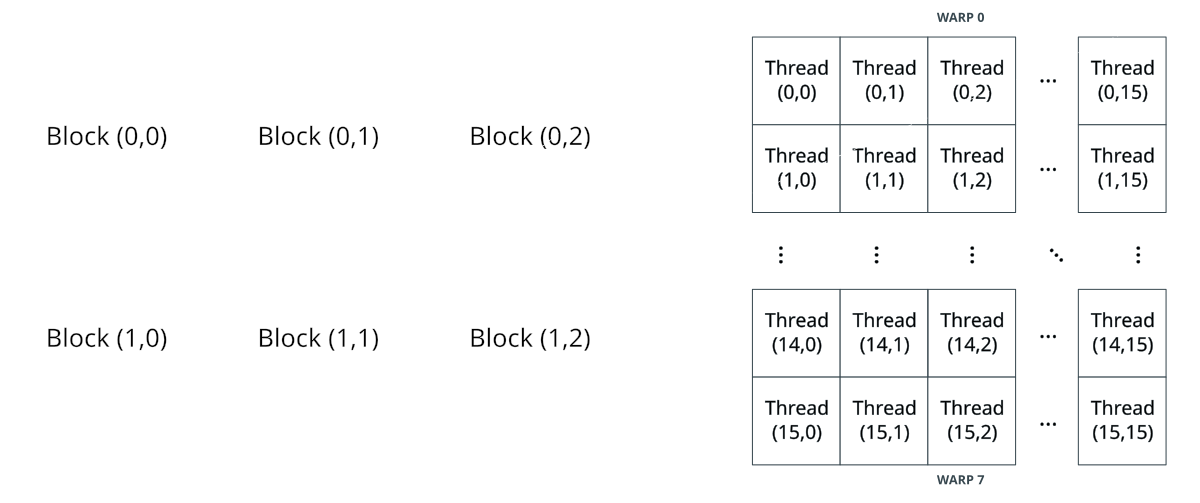
\includegraphics[width=.8\linewidth]{gfx/cudagrid}
	\caption[$2\times3$ grid with $16\times16$ blocks]{$2\times3$ grid with $16\times16$ blocks}
	\label{fig:cudagrid}
\end{figure}

An example configuration of the \ac{CUDA} device can be seen on \autoref{fig:cudagrid}, where 6 two dimensional blocks are arranged on the grid in two rows and three columns. Every block has 256 threads, arranged on a 16$\times$16 matrix.

The shape of the \ac{CUDA} grid and blocks were customizable by the user, but the warps were automatically created by \ac{CUDA}, picking up always sets of successive 32 threads, going first through the $X$ axis, then through the $Y$ axis and finally through the $Z$ axis.

This section studies how the grid and blocks were shaped on our software and the implemented parallelized code, as well as some fine-tuning techniques used to speed up the computations.

\subsubsection*{Device Setup}

The configuration of the grid for a ray tracer seemed natural. As we were working with images, which are simply two dimensional matrices, the grid was shaped as a two dimensional matrix, where every thread computed the geodesic corresponding to a pixel.

The important question was how to configure the pixels between the blocks; \ie, how to define the number of blocks per column and per row in the grid.

The simplest answer was to define one dimensional blocks of a fixed size that extend along the rows of the image. The very first implementation of the ray tracer used this configuration, but the speed up against the \ac{CPU} implementation was very poor.

The branch divergence was guilty of the poor performance: along a row of the image, the behaviour of the corresponding geodesics was very different, and the so-called \emph{warp divergence} occurred: in a warp, which in this configuration was defined along the rows of the image, all threads executed the same instruction at the same time; if the control flow varied between the threads in a warp, some of them would be idle, which caused a great loss of parallel efficiency.

This was avoided by designing a configuration that ensured, or at least that facilitated, that all the threads in a warp executed the same exact code without branch divergence. In our case, this meant that the geodesics hitting the pixels in a warp should have followed a nearby path.

However, without knowing a priori the origin of the geodesics, we could only guess which pixels had similar geodesics. The configuration design followed then this sensible guess: \emph{nearby pixels are hit by geodesics with nearby origins}.

From this assumption, we designed warps as squared as possible, configuring the blocks to have an integer number of warps. This resulted in the following configuration:
\begin{enumerate}
	\item Each block had $8\times8$ threads; \ie, two warps of $8\times4$ threads were located per block. See \autoref{fig:warpconf}.
	\begin{figure}[bth]
		\myfloatalign
		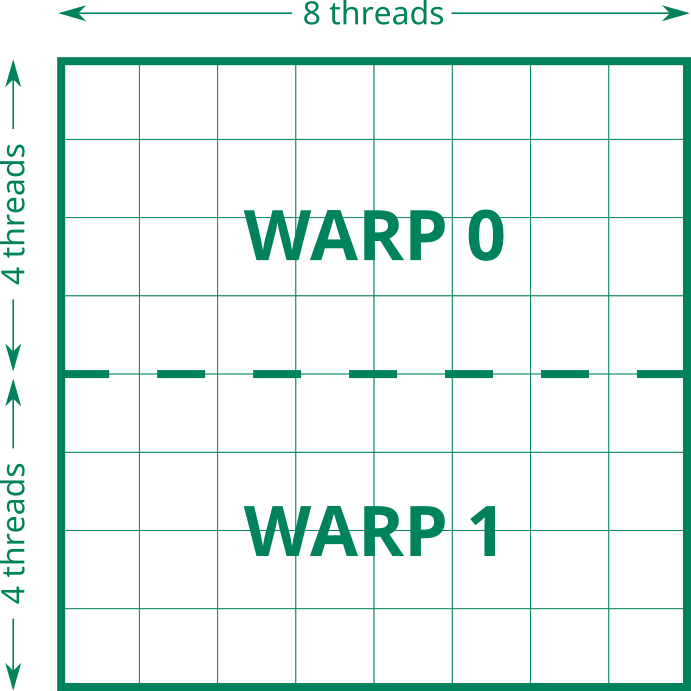
\includegraphics[width=.3\linewidth]{gfx/warpconf.png}
		\caption[Raytracer block configuration]{Raytracer block configuration}
		\label{fig:warpconf}
	\end{figure}
	\item The grid size was dynamically computed using the image size provided by the user. The number of rows and columns of the grid were computed with the following formulas:
	\begin{equation*}
	G_C = \left \lfloor{\frac{I_C - 1}{B_C} + 1}\right \rfloor, \qquad
	G_R = \left \lfloor{\frac{I_R - 1}{B_R} + 1}\right \rfloor,
	\end{equation*}
	where $G_C$ and $G_R$ are the number of blocks per column and per row, $I_C$ and $I_R$ are the columns and rows of pixels of the image and $B_C = B_R = 8$ are the number of columns and rows of a block. These formulas ensured we had enough threads to compute each pixel. The remaining threads, which did not have any geodesic to compute, were idle during all the program execution.
\end{enumerate}

\subsubsection*{CUDA Kernels}

The main function executed by \ac{CUDA} on the \ac{GPU} is called the \emph{kernel}. Our implementation had three kernels, where every thread was identified with a pixel via its unique identifier in the \ac{CUDA} device. The kernels were:
\begin{enumerate}
	\item \lstinline{setInitialConditions()}: it was the kernel to compute the initial conditions for every pixel, as designed in \autoref{sec:initcond}. From the pixel coordinates, it computed the corresponding pair $(\vartheta_{cs}, \varphi_{cs})$.
	\item  \lstinline{kernel()}: it was the main kernel. It received the initial conditions for every pixel and the final time until which the \ac{ODE} system was integrated. It computed the origin of each geodesic, \ie, the pair $(\vartheta', \varphi')$, using the design described at \autoref{sec:numerical}, while continuously checking for collisions with the accretion disk.
	\item \lstinline{generate_image()}: it was an auxiliary kernel to map textures into the images. It received the origin of the geodesic corresponding to each pixel in the image and mapped it to a pixel in the provided texture.
\end{enumerate}

\subsubsection*{Optimizations}

The computational bottleneck of the ray tracer was the \ac{ODE} solver. In particular, the computation of the right hand side of the system ---in terms of the \autoref{sec:numerical}, the function $f(y,t)$---, which involved a lot of operations, some of them really expensive, as the \lstinline{sin()} and \lstinline{cos()} functions.

This chunk of code was highly optimised, pre-computing all repeated operations and using efficient implementations such as the \lstinline{sincos()} function. The derivatives on equations \ref{eq:eqsmotionp}, \ref{eq:eqsmotionpr} and \ref{eq:eqsmotionpt} were expressed in their most elementary terms and all common quantities between them were also pre-computed. To optimise the memory access time, the thread's local memory was used whenever it was possible.

Furthermore, a specific issue was taken into account: the \ac{ILP}. It is clear that a single thread cannot keep the \ac{GPU} busy, so the device schedules threads and instructions in such a way that the \ac{GPU} is always busy.

One way of helping the \ac{CUDA} scheduler to maximize the device occupancy is to design the code optimising the \ac{ILP}. All the ray tracer implementation was coded in such a way that independent instructions were together, whereas dependent ones were as far as possible one of the other. This let the scheduler issue instructions in parallel without having to wait for dependent computations to finish. In particular, the code of the computation of $f(y,t)$ was deeply studied in order to maximize the \ac{ILP}.

\subsubsection*{Initial Conditions Computation}

The initial conditions computation was implemented as a kernel on the \lstinline{raytracer.cu} file.

It received a pointer to two allocated sections of memory in the device: one to store the output of the initial conditions and another to store the output of the computation of the conserved quantities $b$ and $q$.

Each thread solved the formulas obtained in \autoref{sec:pinhole}: equations \ref{eq:pinhole1} and the ones obtained in \autoref{sec:initcond}, and stored the computed values in the pointed sections of the memory.

\subsubsection*{Ray Tracing}

The ray tracing kernel implemented the main logic of the software: it executed the \ac{RK} solver while continuously checking for collisions with either the disk or the black hole, following the design on \autoref{sec:numerical}.

It received a pointer to an allocated section of the memory where the initial conditions of the system were stored. After solving the \ac{ODE} system, it rewrote this buffer to provide the user with the final \ac{BL} coordinates of the considered geodesics.

An auxiliary buffer was used in order to known if a given geodesic had hit the disk, had fallen into the black hole or if it pointed to the celestial sphere.

\subsubsection*{Texture Mapping}

The texture mapping was a simple kernel implemented in the \lstinline{image_transformation.cu} file. It received the final computed solution of the \ac{ODE} system, a pointer to a section of the memory where the textures pixels were assumed to be stored along with the size of the textures and a pointer to another previously allocated section of memory where the final pixels of the image would be stored.

It then computed the texture mapping and output the result to the final image.




















\section{Results}
\label{chapter:results}

The implemented software fulfilled the objectives and requirements set at the design stage. It was able to ray trace arbitrary geodesics from the point of view of a camera, arbitrarily placed on a Kerr spacetime, allowing the user to plot the simulated geodesics both as photographies and as three dimensional projections.

\begin{figure}[bth]
	\myfloatalign
	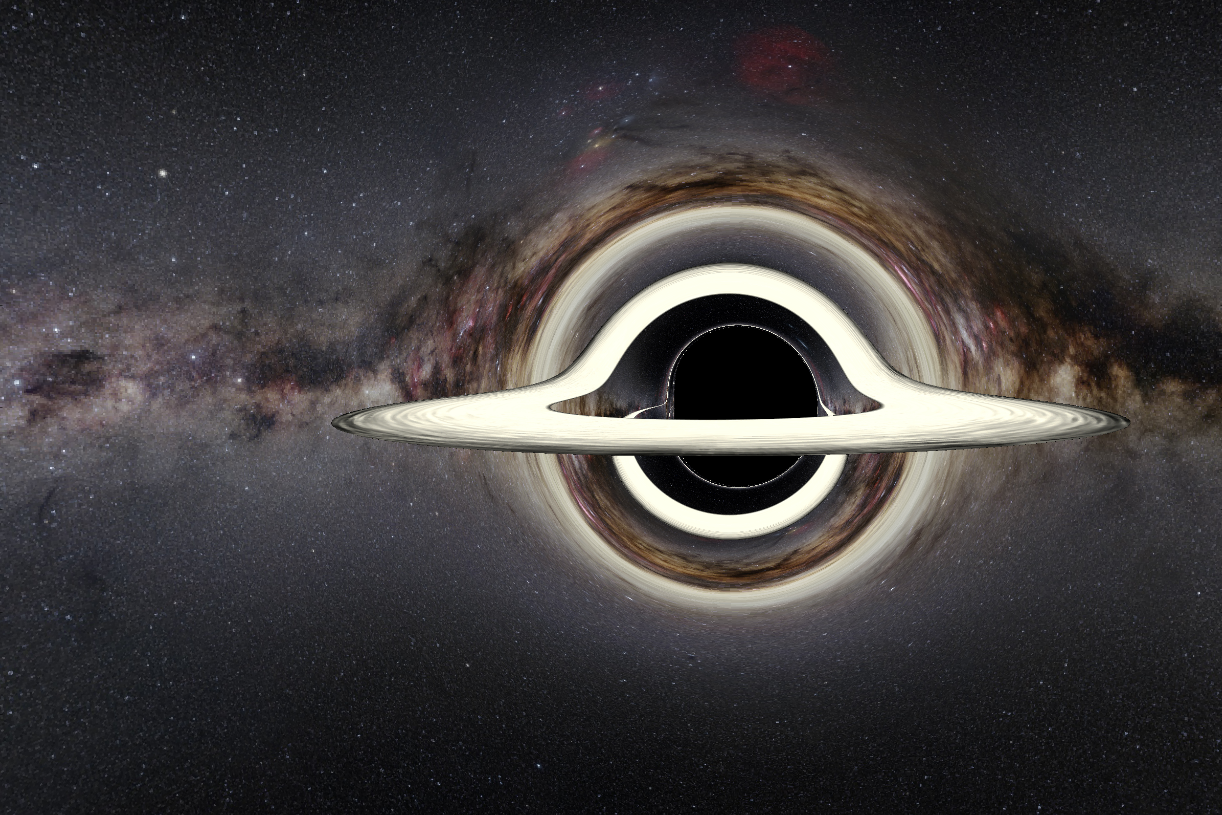
\includegraphics[width=\linewidth]{gfx/bh_texture_disk}
	\caption[Cinematographic textured image]{Cinematographic textured image}
	\label{fig:blackhole}
\end{figure}

Furthermore, the implemented \ac{ODE} solver accuracy was successfully tested, while the speed up of the \ac{GPU} parallelized code was proved to be very high.

\subsection{Ray Tracer Features}

The ray tracer generated images with a wide range of possibilities: it simulated photographies made with a common camera near the black hole, an accretion disk could be added to show the curvature of the light near its surroundings and arbitrary textures could be configured, letting the user experiment with the light and the distortions produced by the greatly curved spacetime near the Kerr black hole.

\autoref{fig:blackhole} is one example of a fully featured image with a cinematographic look: the celestial sphere was textured with an image of the Milky Way; an accretion disk around the black hole was added and a texture on the disk was rendered.

The rendered images could also be plotted as three dimensional projections, letting the user observe the paths followed by the geodesics, as seen on \autoref{fig:3dprojection}. Blue lines represent geodesics that come from the celestial sphere, red lines are geodesics that never existed, as they would have originated inside the black hole's horizon; green lines are the geodesics whose origin is on the accretion disk.

The computed information could be rendered independently as a three dimensional projection or as an image. \autoref{fig:3dprojectionimage} shows the photography whose three dimensional representation was depicted on \autoref{fig:3dprojection}.

\begin{figure}[bth]
	\myfloatalign
	\subfloat[Top view.]
	{\frame{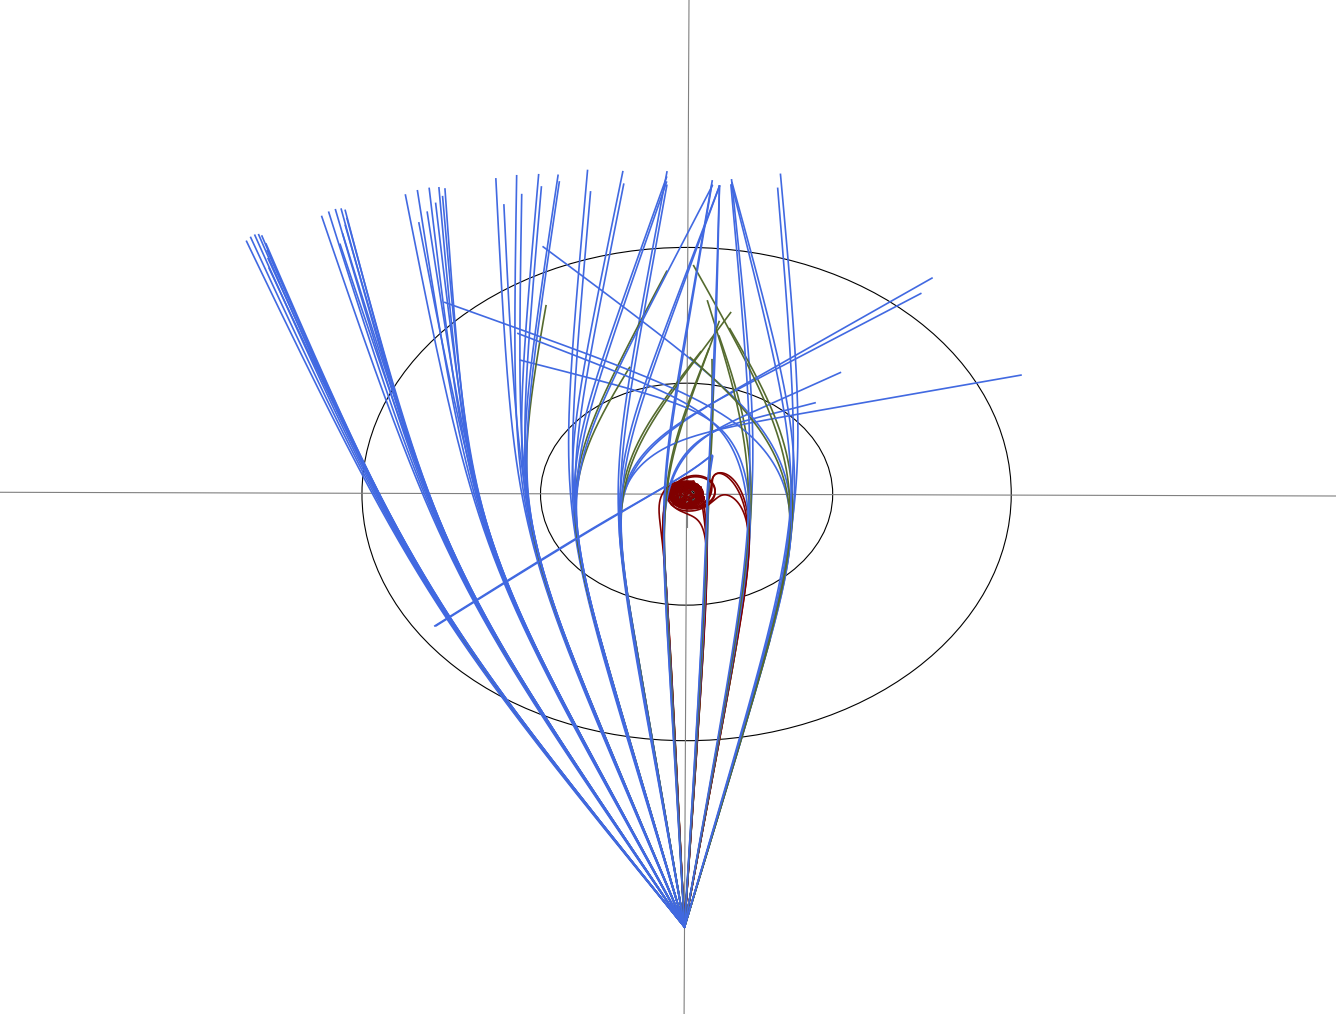
\includegraphics[width=.45\linewidth]{gfx/3d_01_top}}} \quad
	\subfloat[Right view.]
	{\frame{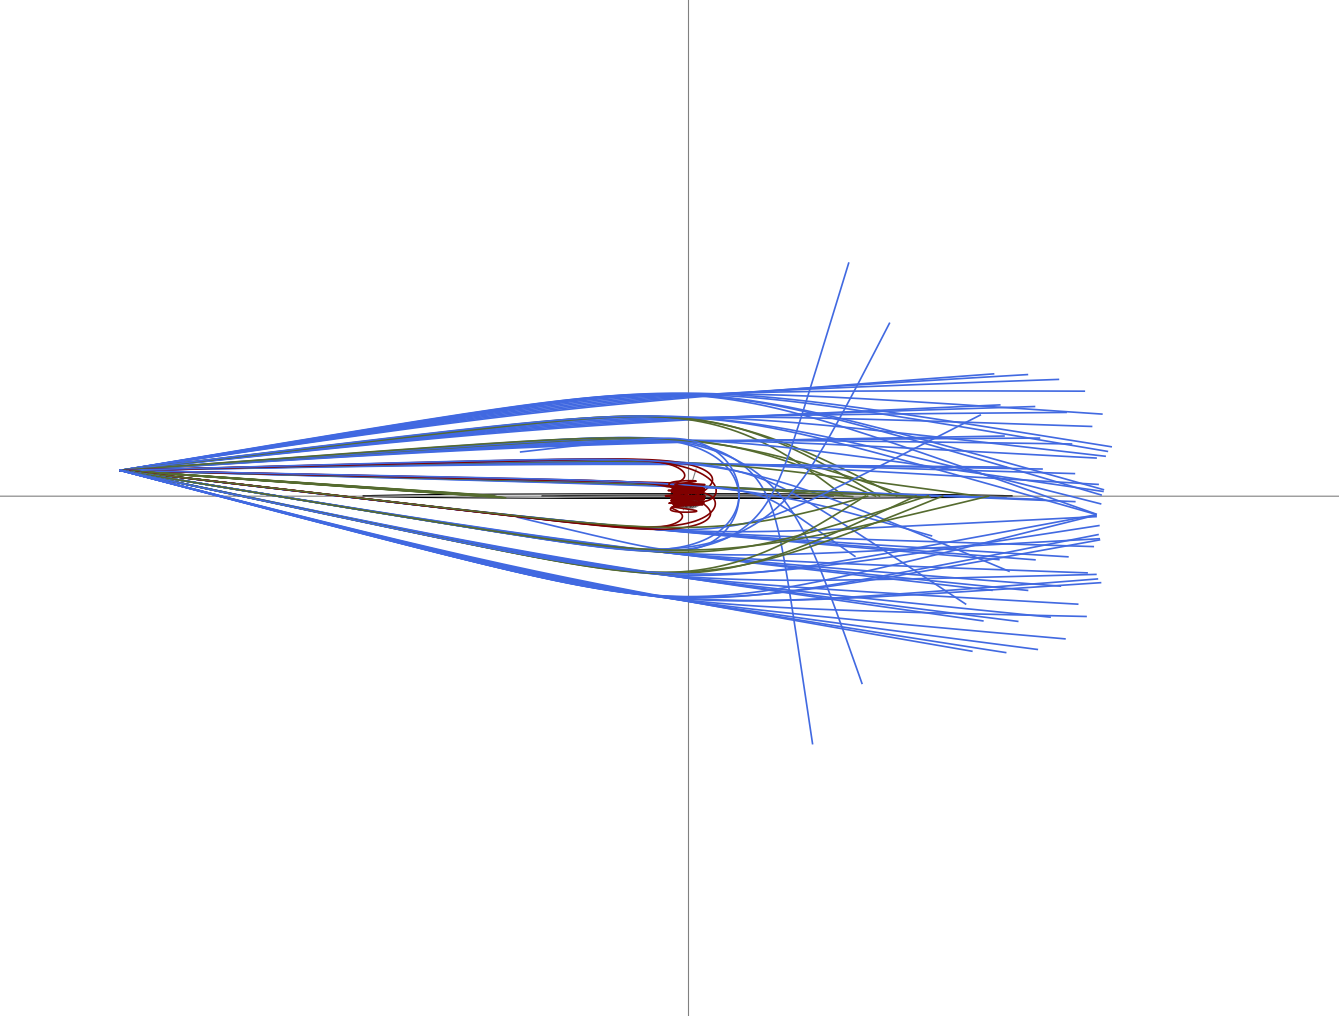
\includegraphics[width=.45\linewidth]{gfx/3d_01_right}}} \\
	\subfloat[Perspective view from behind.]
	{\frame{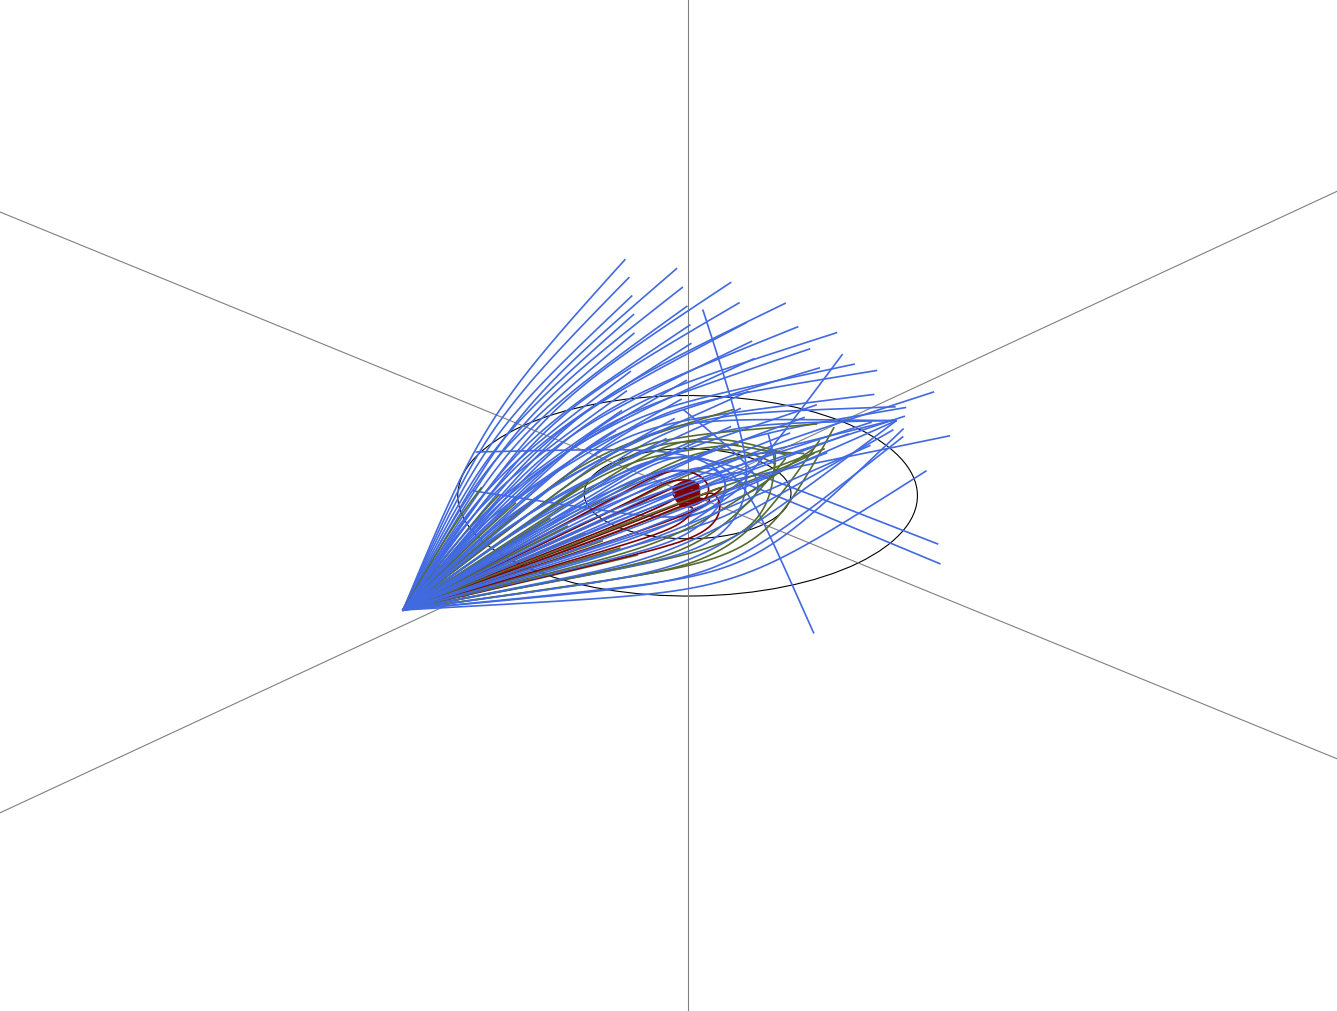
\includegraphics[width=.45\linewidth]{gfx/3d_01_perspective1}}} \quad
	\subfloat[Perspective view from the front side.]
	{\frame{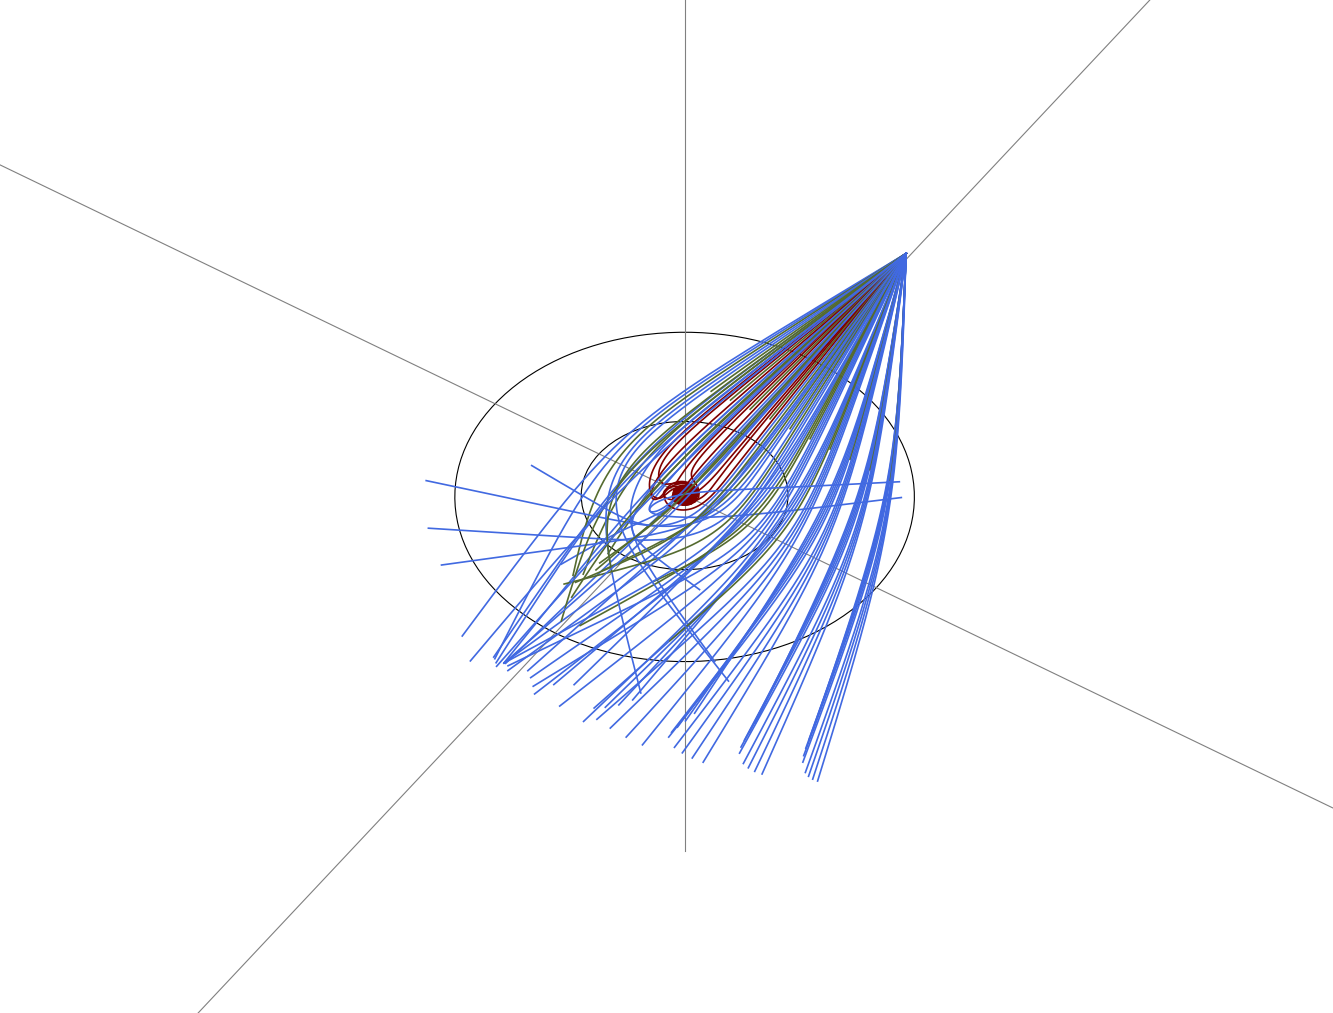
\includegraphics[width=.45\linewidth]{gfx/3d_01_perspective2}}}
	\caption[3D representation of the geodesics]{3D representation of the geodesics.}\label{fig:3dprojection}
\end{figure}

\begin{figure}[bth]
	\myfloatalign
	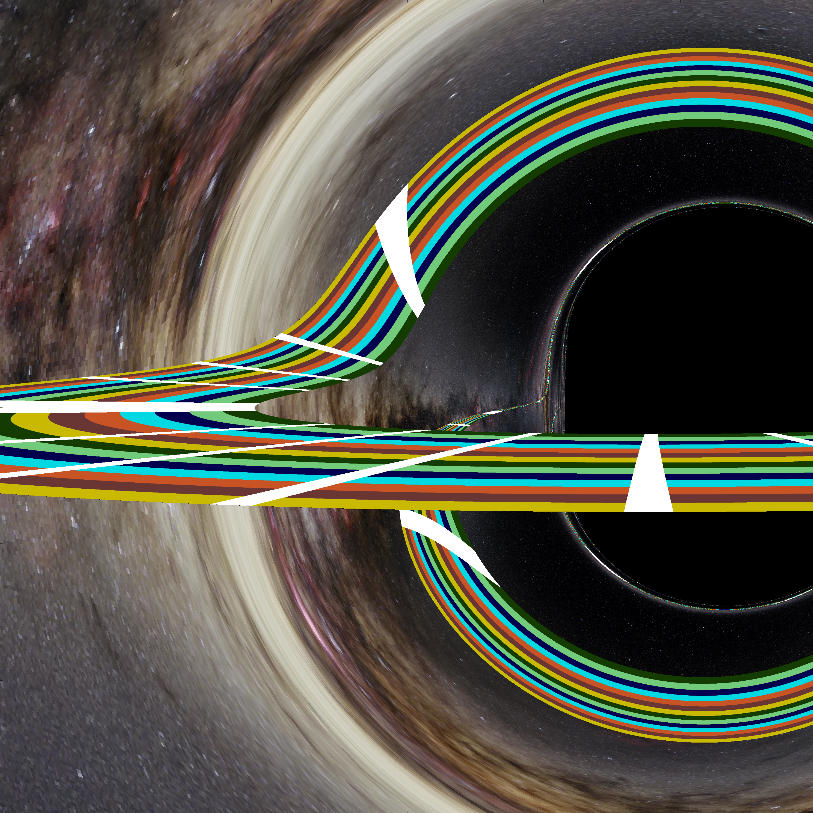
\includegraphics[width=.5\linewidth]{gfx/3d_01_image}
	\caption[Photography from a 3D scenario]{Photography of the 3D scenario rendered in \autoref{fig:3dprojection}}
	\label{fig:3dprojectionimage}
\end{figure}

\subsection{Computational Results}

\subsubsection*{Runge-Kutta Solver Accuracy}

The \ac{RK} solver was tested not only against the geodesics \ac{ODE} system, but against usual functions whose analytic expression was known. This test was done to prove that the solver was accurate and to study the behaviour of the automatic step size computation.

\autoref{fig:stepsize} shows the behaviour of the \ac{RK} solver on the Airy function $Bi(x)$. The orange line is its analytic expression, while the blue points are the solution computed by the \ac{RK} solver of the associated \ac{ODE}: $\frac{d^2y}{dx^2} - xy = 0$.

\begin{figure}[bth]
	\myfloatalign
	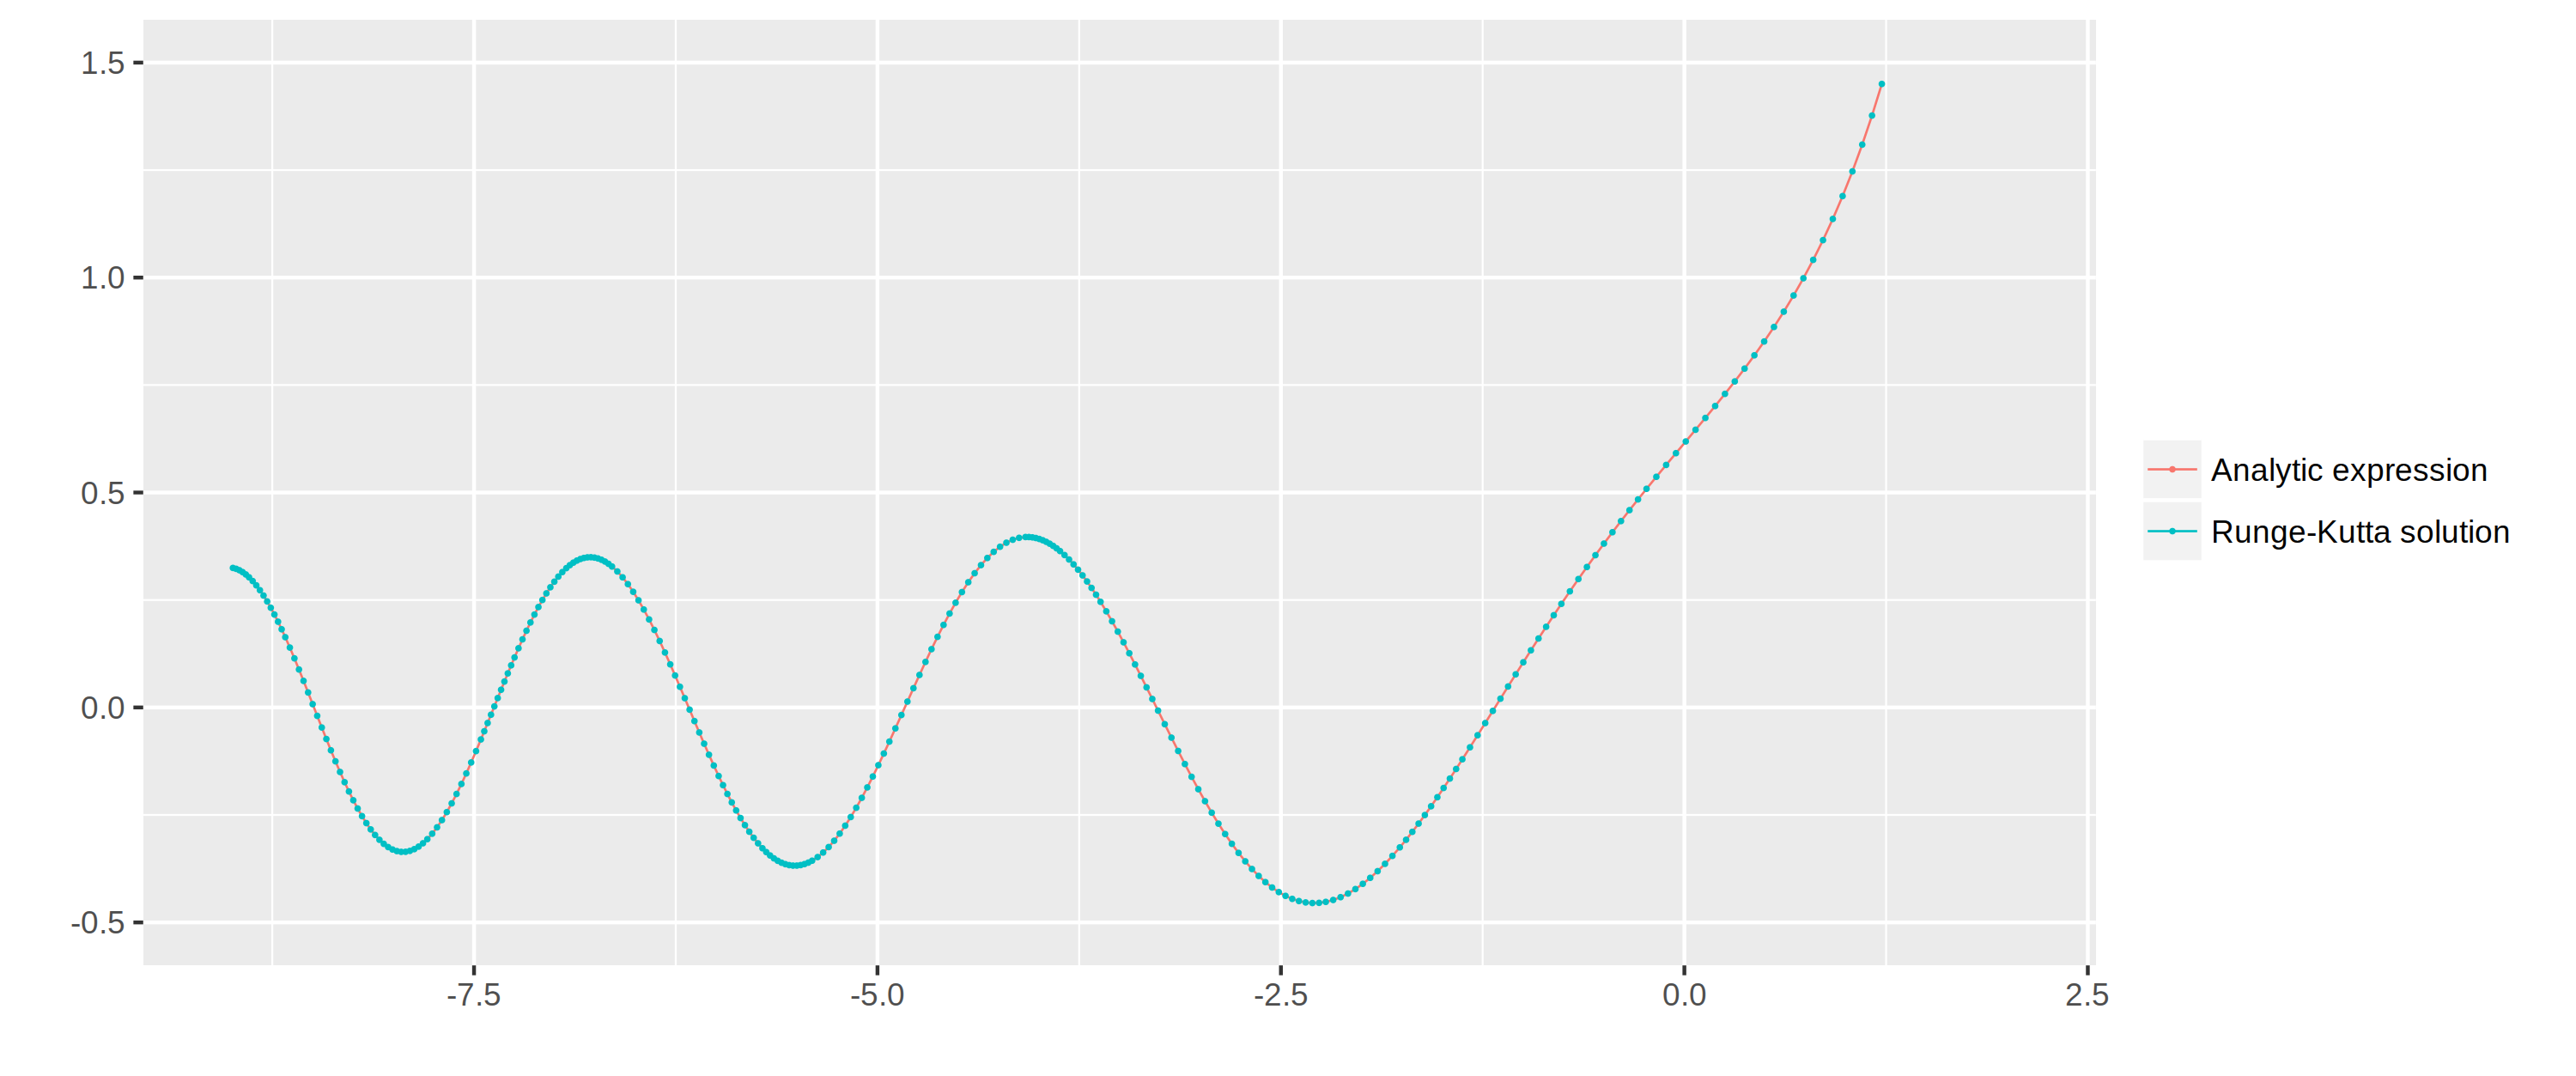
\includegraphics[trim={4cm 0 12cm 5cm},clip,width=.5\linewidth]{gfx/analytic}
	\caption[Solver in an analytic function]{\ac{RK} solver in an analytic function}
	\label{fig:stepsize}
\end{figure}

The automatic step computation algorithm worked smoothly: when the function could be approximated as a straight line, the step was very large. In intervals where the function curvature changed rapidly, the algorithm reduced the step in order to better approximate the function value.

This behaviour was also seen on the geodesics \ac{ODE} system. \autoref{fig:kretschmann} shows the normalized values of four quantities: the Kretschmann invariant, which measures the curvature of the spacetime; the distance to the black hole; the value of $\vartheta$ and the step computed by the automatic step algorithm. When the particle approached the black hole, the Kretschmann increased, the system became unstable and so the algorithm reduced the step size in order to better approximate its value. In fact, both the step line and the radius line were very similar, showing the correlation between the computed step and the distance to the black hole centre.

\subsubsection*{Efficiency}

Regarding the efficiency of the ray tracer, a benchmark against a \ac{CPU} implementation was done. The \ac{CPU} implementation had essentially the same code that the \ac{GPU}-parallelized version, except for the obvious changes that were made to adapt the code to the \ac{CUDA} grid.

\autoref{fig:speedup} shows two benchmarks using both versions of the ray tracer: one with a Kerr spacetime where the black hole had a spin of $a = 0.0001$ and another one where the spin was $a = 0.999$. For both benchmarks, the speed up is plotted: the line represented for each of them shows how many times faster was the \ac{GPU}-parallelized version against the \ac{CPU} implementation.

\begin{figure}[bth]
	\myfloatalign
	\subfloat[Step, $r$, $\vartheta$ and Kretschmann]
	{\label{fig:kretschmann}%
		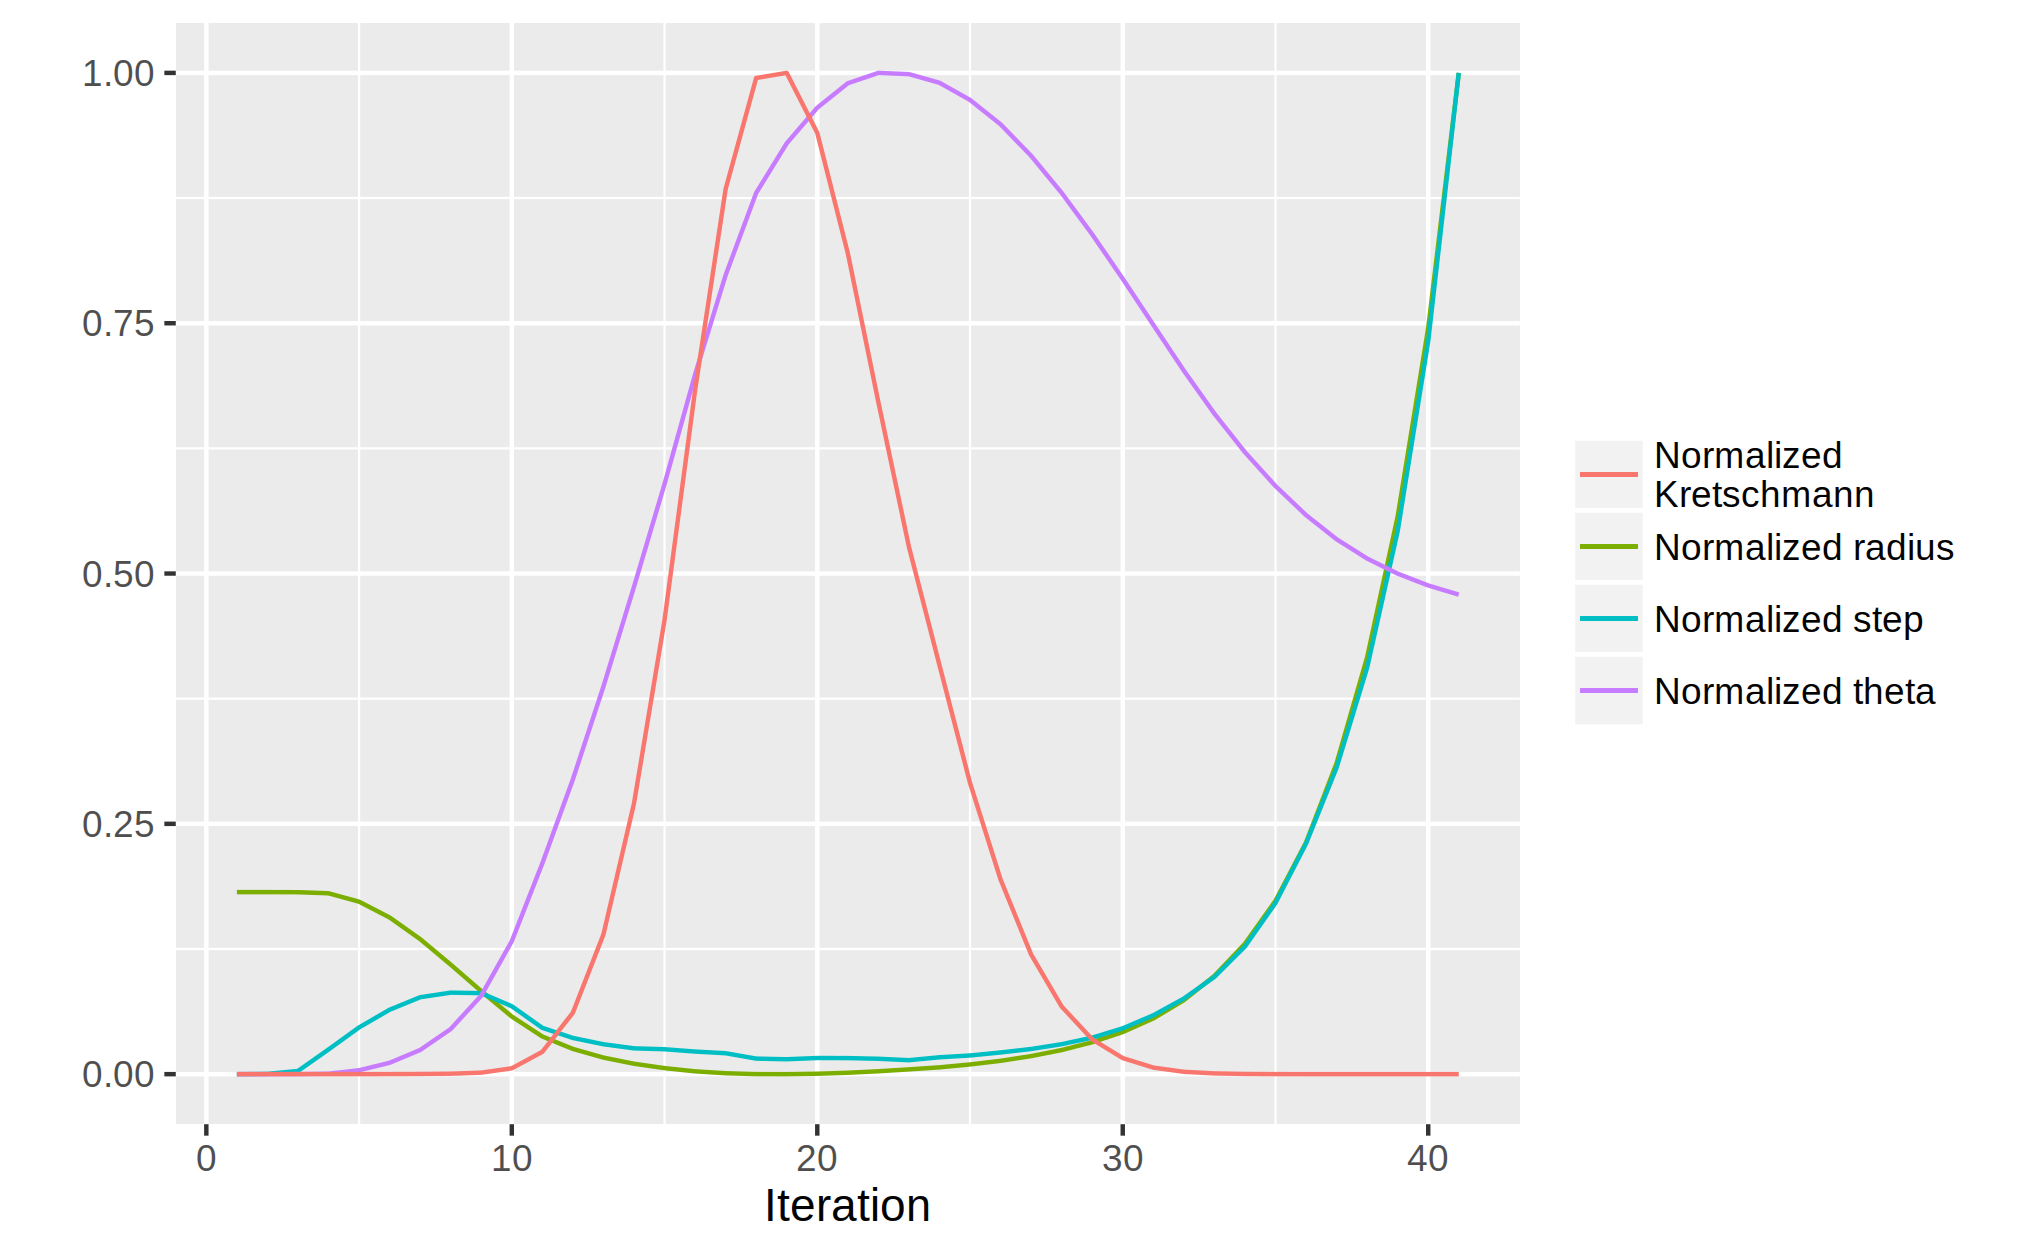
\includegraphics[width=.45\linewidth]{gfx/kretschmann}} \quad
	\subfloat[Speed up with different spins]
	{\label{fig:speedup}%
		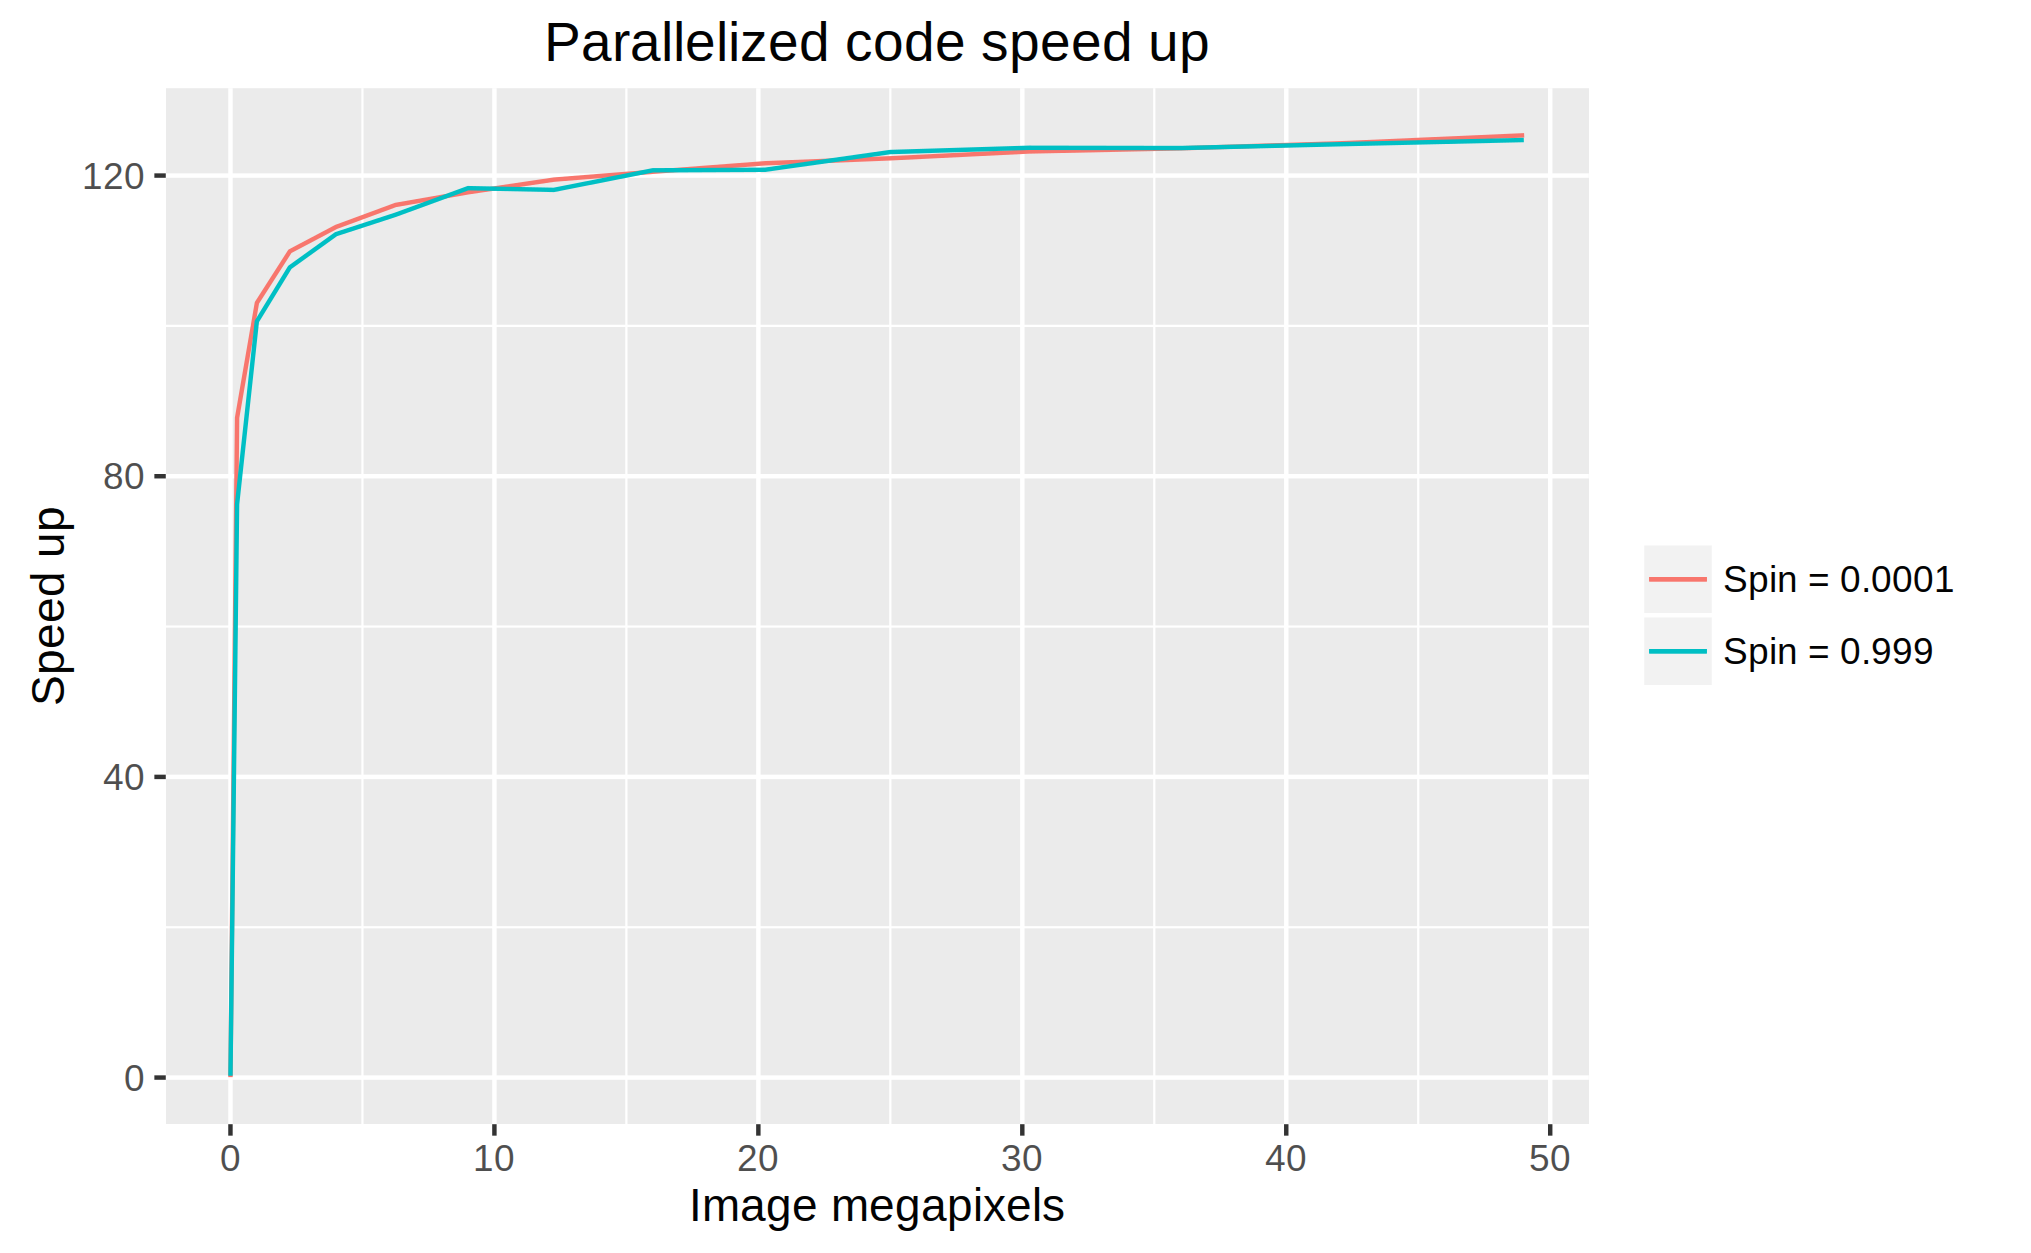
\includegraphics[width=.45\linewidth]{gfx/speedup}}
	\caption[Benchmark results]{Benchmark results}\label{fig:benchmark}
\end{figure}


The speed up increased at a great speed when the number of pixels were augmented. It stabilized around 20 megapixels with a speed up of about $125$. The mean speed up equalled $108.5$ on the low spin case, whereas in the high spin case equalled $107.2$. The maximum speedup obtained equalled $125.3$ on the first case, with a maximum speed up of $124.7$ on the second.

The speed up seemed to be stable against changes on the spin. This figure summarises the power of \ac{GPGPU}, that can increase the performance of a piece of software by several orders of magnitude.


\subsection{Scientific Results}

The main objective of the ray tracer implementation was to serve as a tool for scientists to study properties of the Kerr spacetime. This section summarises some of these interesting features.

\subsubsection*{Spin}

We generated images without any accretion disk or textures, obtaining binaries images where the black pixels represented the shadow of the black hole and the white pixels the celestial sphere. \autoref{fig:shadow} shows four images taken with the same camera, which was placed on the equatorial plane, with a null speed and focusing the black hole's centre. The only change between images was the black hole's spin. The first one shows a perfect sphere, where the Kerr metric can be reduced to Schwarzschild metric. \autoref{fig:shadow-b} and \autoref{fig:shadow-c} show that there was a slight change on the virtual position of the shadow and, although it is difficult to see, the shape was not circular. The edge case, depicted on \autoref{fig:shadow-d}, made clear the effect of a large spin on the shadow of the black hole. As it curved the geodesics rapidly, it was seen slightly moved to the right and with a flat side on the left.

\begin{figure}[bth]
	\myfloatalign
	\subfloat[Spin $\approx$ 0]
	{\frame{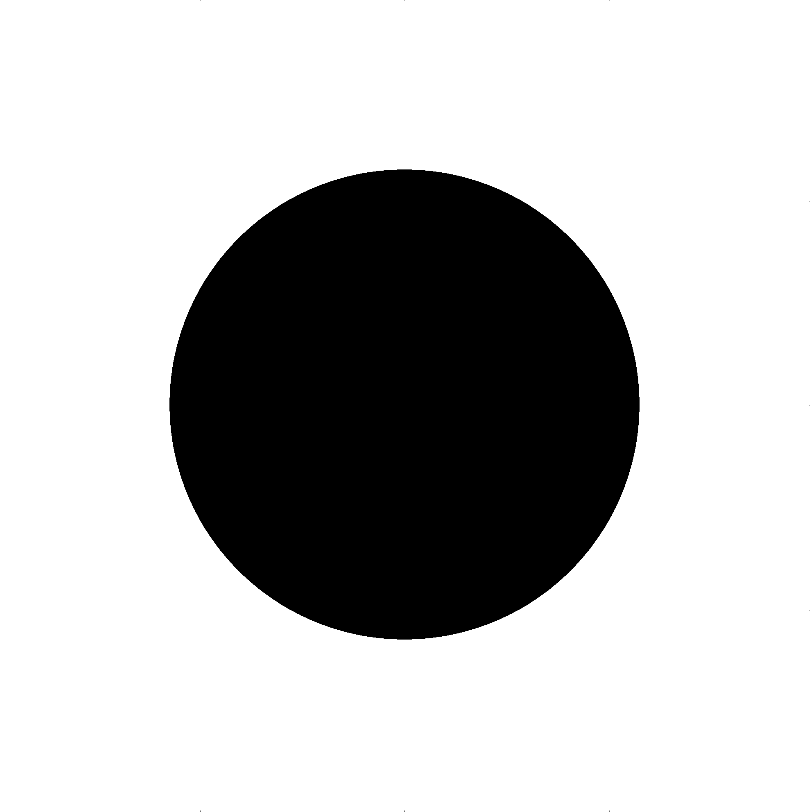
\includegraphics[width=.3\linewidth]{gfx/bh_shadow_spin0001}}} \quad
	\subfloat[Spin = 0.25]
	{\label{fig:shadow-b}%
		\frame{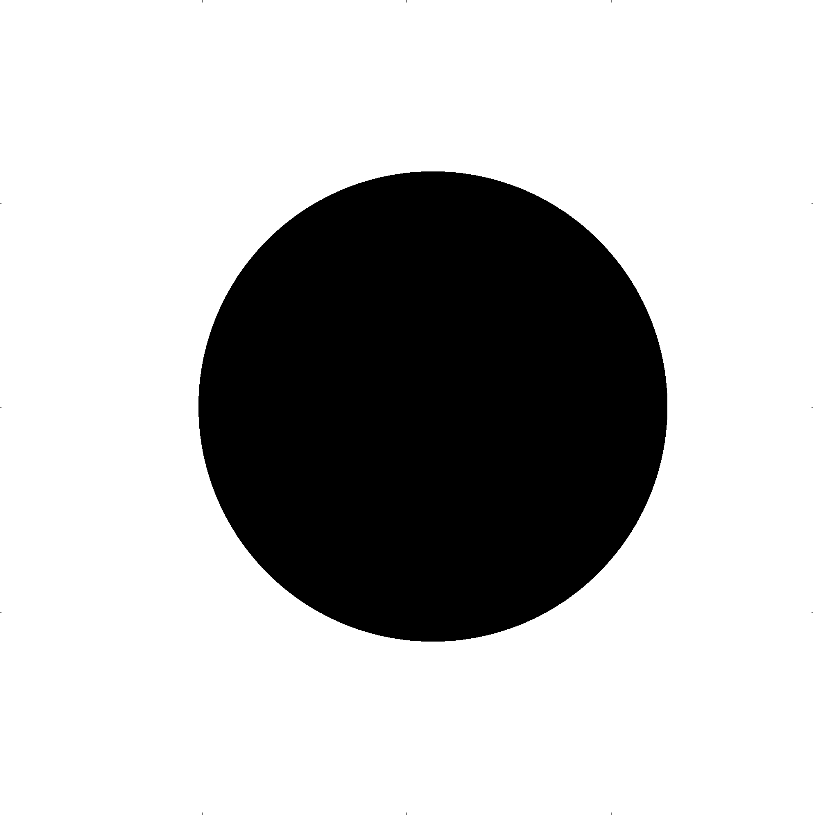
\includegraphics[width=.3\linewidth]{gfx/bh_shadow_spin25}}} \\
	\subfloat[Spin = 0.75]
	{\label{fig:shadow-c}%
		\frame{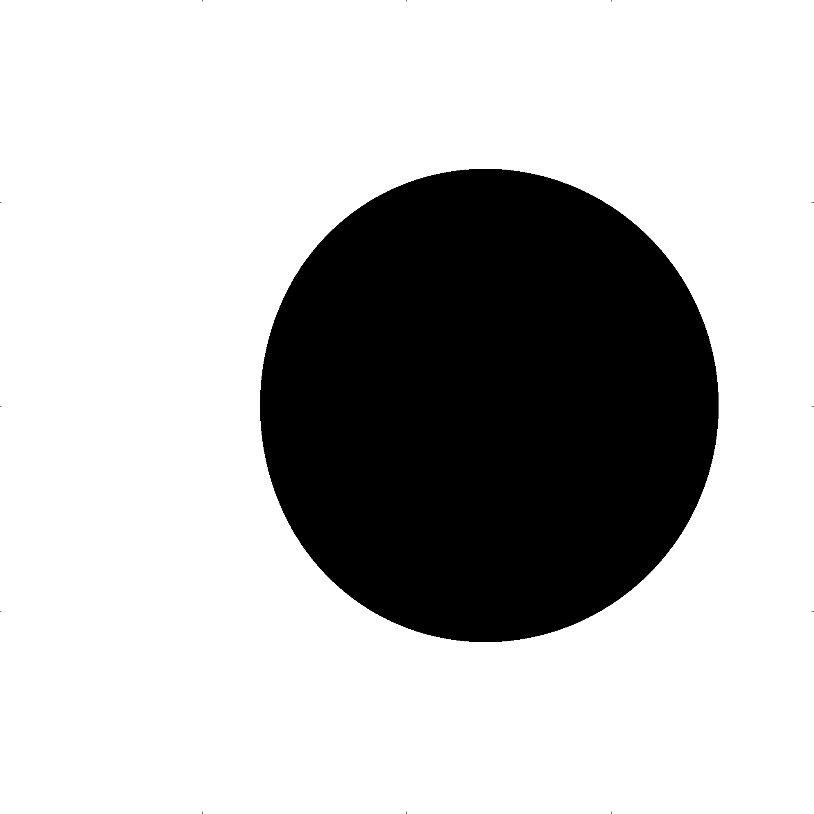
\includegraphics[width=.3\linewidth]{gfx/bh_shadow_spin75}}} \quad
	\subfloat[Spin $\approx$ 1]
	{\label{fig:shadow-d}%
		\frame{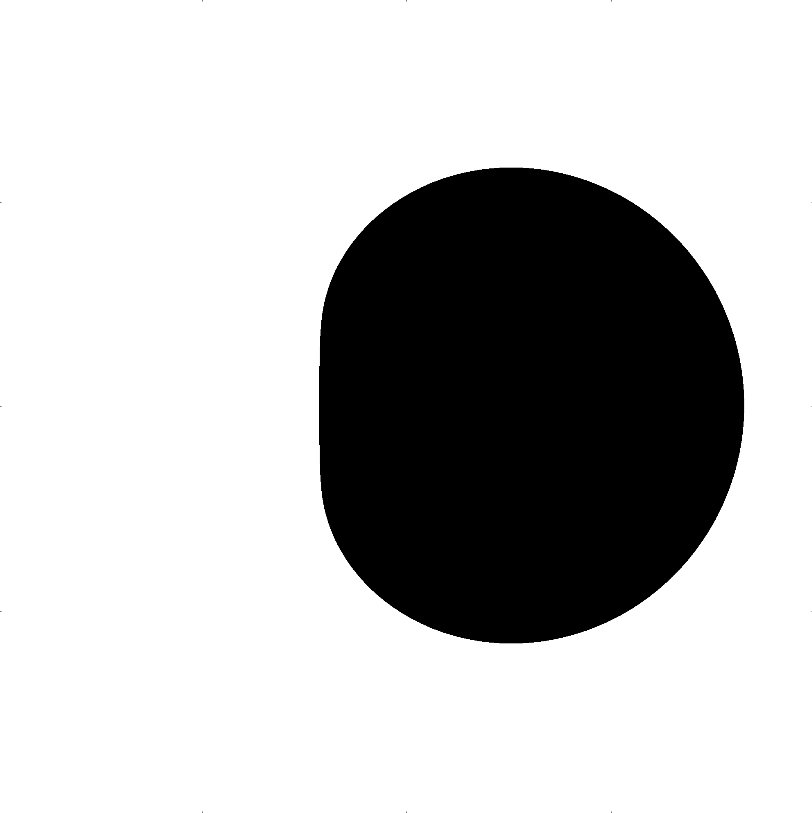
\includegraphics[width=.3\linewidth]{gfx/bh_shadow_spin999}}}
	\caption[Black hole shadow for different spins]{Black hole shadow for different spins}\label{fig:shadow}
\end{figure}

We also studied what happens with straight lines that fall inside the black hole. Imagine an accretion disk around the black hole, with its inner radius minor than the horizon radius and an infinite outer radius. If we visualize this disk with a patched texture made by white and red squares, we can see the effect of the spin on its shape.

\autoref{fig:xmas-a} shows the most simple version of this scenario, where the black hole did not rotate: straight lines falling inside the black hole on the equatorial plane remained intact. Taking this as the base case, we saw what happens when we increase the black hole's spin. \autoref{fig:xmas-b} and \autoref{fig:xmas-c} shows the scenario for spins of $0.25$ and $0.75$. The straight lines started to rotate accordingly with the black hole. On \autoref{fig:xmas-d} ---where the spin nearly equalled 1---, the lines curved greatly when they approach the shadow, and start rotating rapidly when they were close to the horizon.

\begin{figure}[bth]
	\myfloatalign
	\subfloat[Spin $\approx$ 0]
	{\label{fig:xmas-a}%
		\frame{
\includegraphics[width=.3\linewidth]{gfx/bh_xmas_spin0001}}} \quad
	\subfloat[Spin = 0.25]
	{\label{fig:xmas-b}%
		\frame{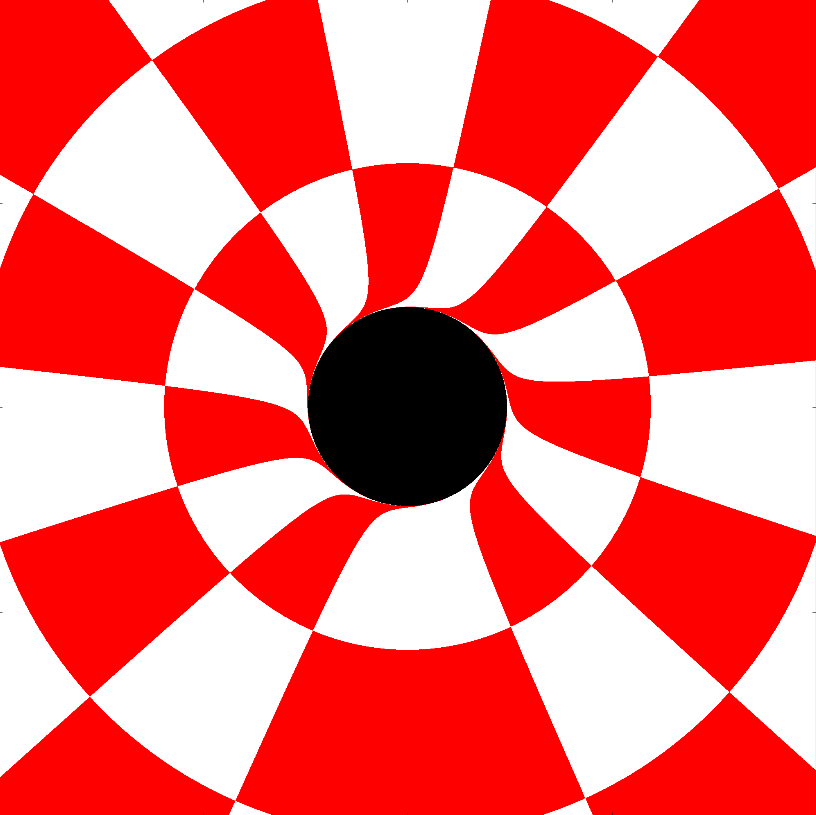
\includegraphics[width=.3\linewidth]{gfx/bh_xmas_spin25}}} \\
	\subfloat[Spin = 0.75]
	{\label{fig:xmas-c}%
		\frame{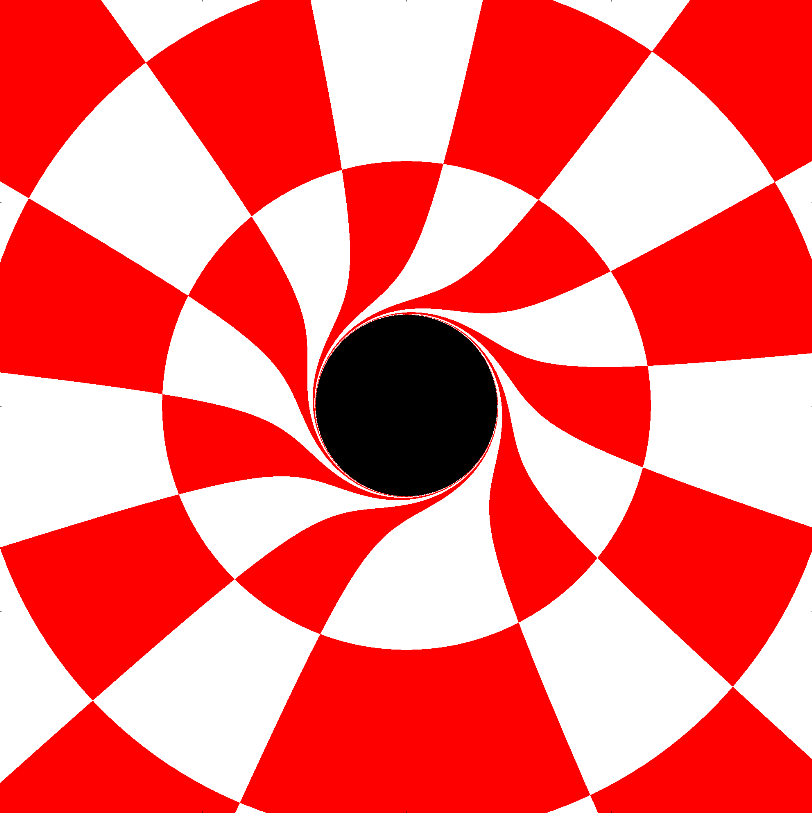
\includegraphics[width=.3\linewidth]{gfx/bh_xmas_spin75}}} \quad
	\subfloat[Spin $\approx$ 1]
	{\label{fig:xmas-d}%
		\frame{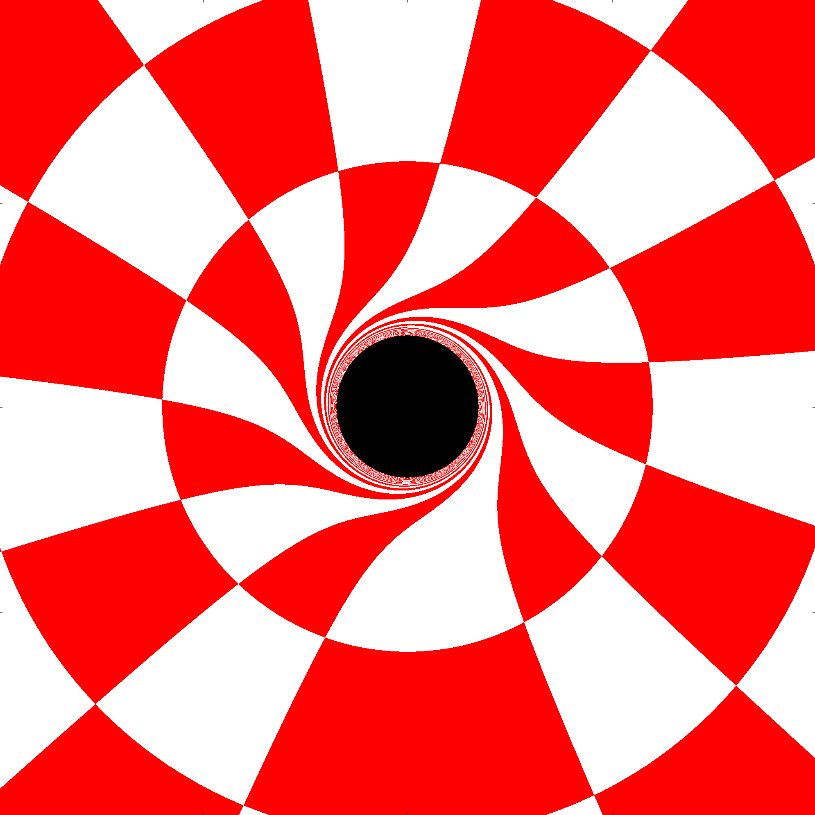
\includegraphics[width=.3\linewidth]{gfx/bh_xmas_spin999}}}
	\caption[Black hole shadow for different spins]{Black hole shadow for different spins}\label{fig:xmas}
\end{figure}

\subsubsection*{Shadow}

One could also map a texture on the black hole's horizon to really know what we are seeing when looking at the shadow. \autoref{fig:texhoriz} shows such an image, where a patched texture drawing the meridians and the parallels was mapped onto the horizon's surface. This image told us that, when we are looking at the shadow of a Kerr black hole, we are seeing the whole surface of the horizon.

\begin{figure}[bth]
	\myfloatalign
	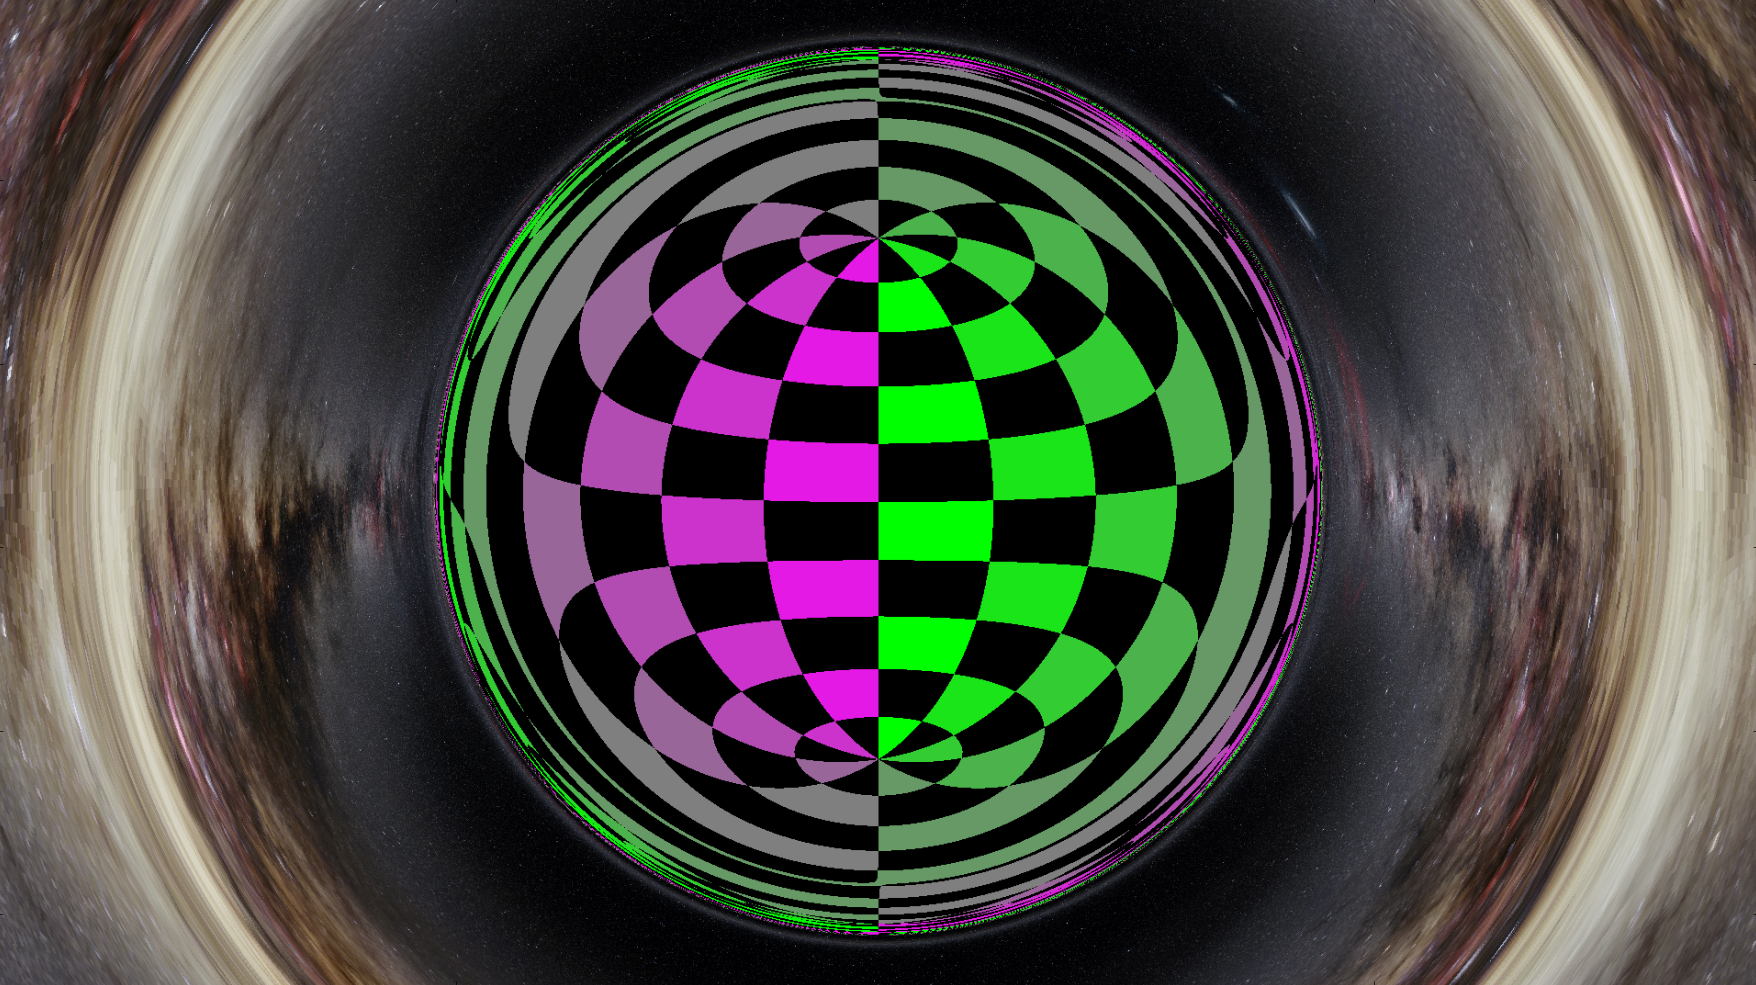
\includegraphics[width=.8\linewidth]{gfx/gridhorizon}
	\caption[Textured horizon]{Textured horizon.}
	\label{fig:texhoriz}
\end{figure}

\subsubsection*{Accretion Disk}

The curvature of the disk around the black hole let us understand the nature of the distortion produced by the spacetime. We saw that the disk bottom is formed by particles that travel below the black hole and hit the disk just at the back of the shadow. A three dimensional projection of a set of these geodesics can be seen on \autoref{fig:under_disk}.

\autoref{fig:insidehalo} shows a set of geodesics that formed the final image of the inner halo. \autoref{fig:upperhalo} shows the intricate paths followed by the geodesics of the upper part of the inner halo, that twist around the black hole, get behind the disk and scatter to cover a great part of the bottom part of the disk. \autoref{fig:wholehalo} summarises all this tour by plotting all geodesics that form the inner halo in just one image.

\begin{figure}[bth]
	\myfloatalign
	\subfloat[Disk bottom]
	{\label{fig:under_disk}%
		\frame{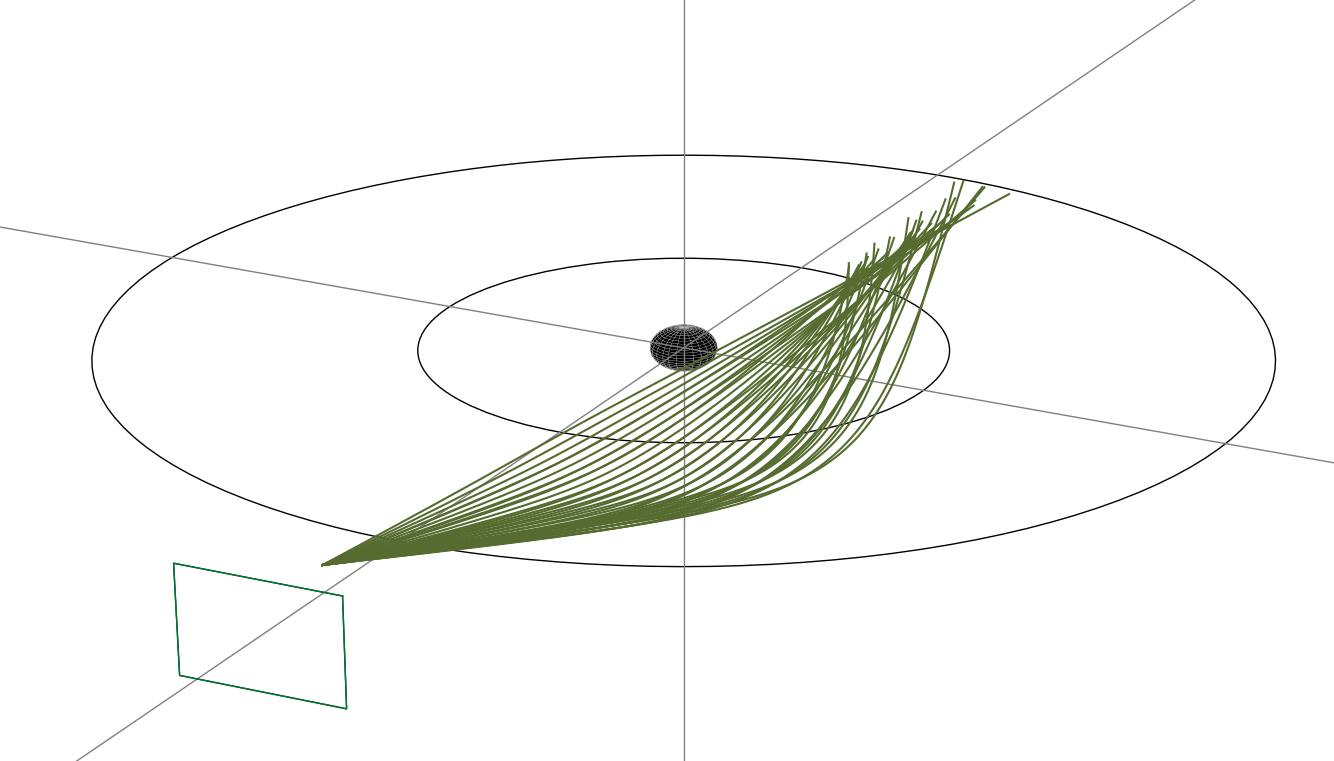
\includegraphics[width=.35\linewidth]{gfx/under_disk}}} \quad
	\subfloat[Inner halo]
	{\label{fig:insidehalo}%
		\frame{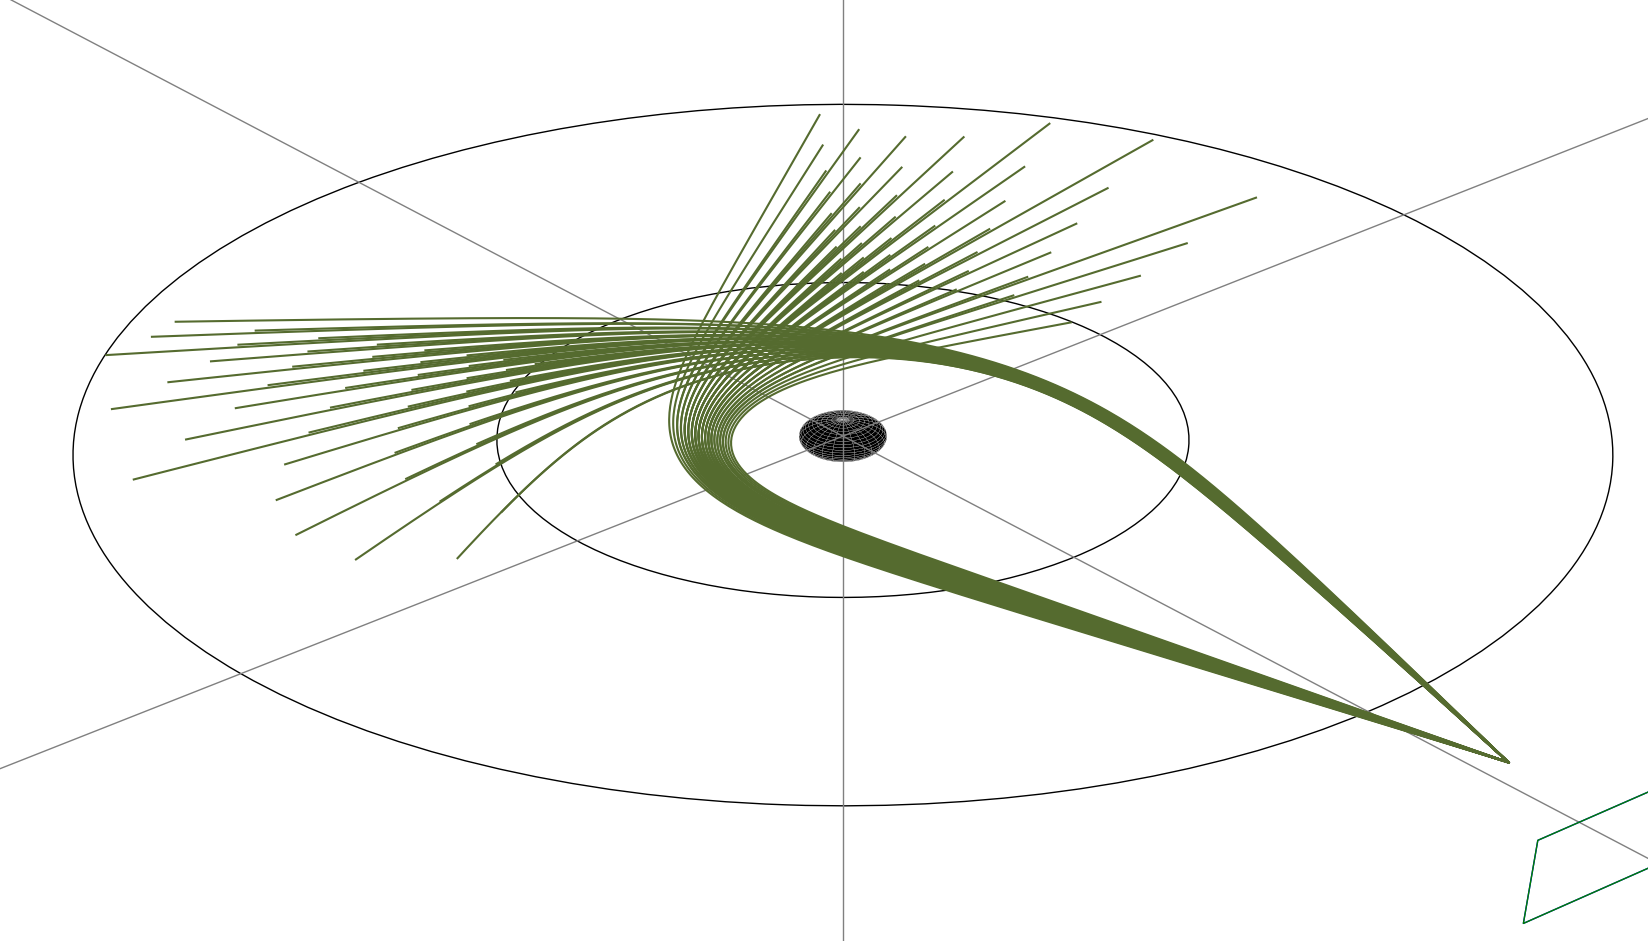
\includegraphics[width=.35\linewidth]{gfx/disk_inside_halo}}} \\
	\subfloat[Upper part of the inner halo]
	{\label{fig:upperhalo}%
		\frame{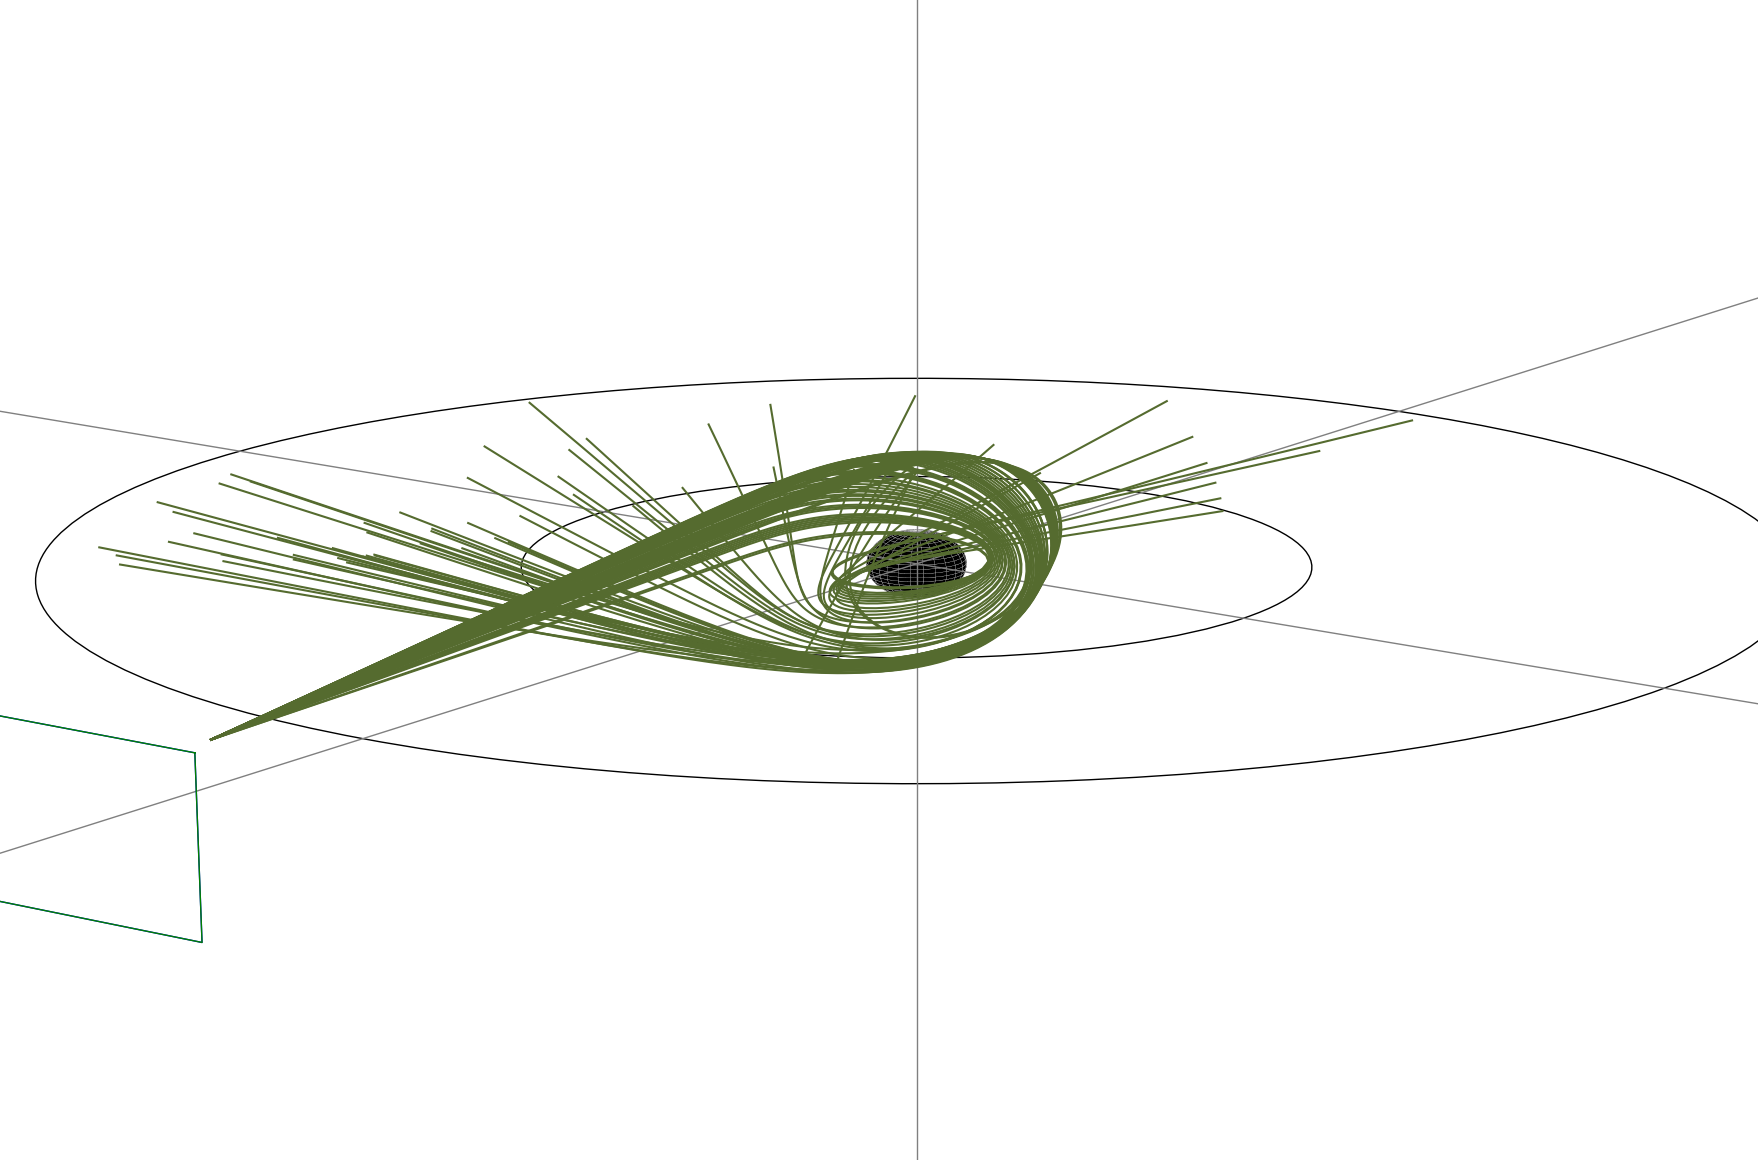
\includegraphics[width=.35\linewidth]{gfx/disk_inside_halo_superior}}} \quad
	\subfloat[Geodesics forming the disk image]
	{\label{fig:wholehalo}%
		\frame{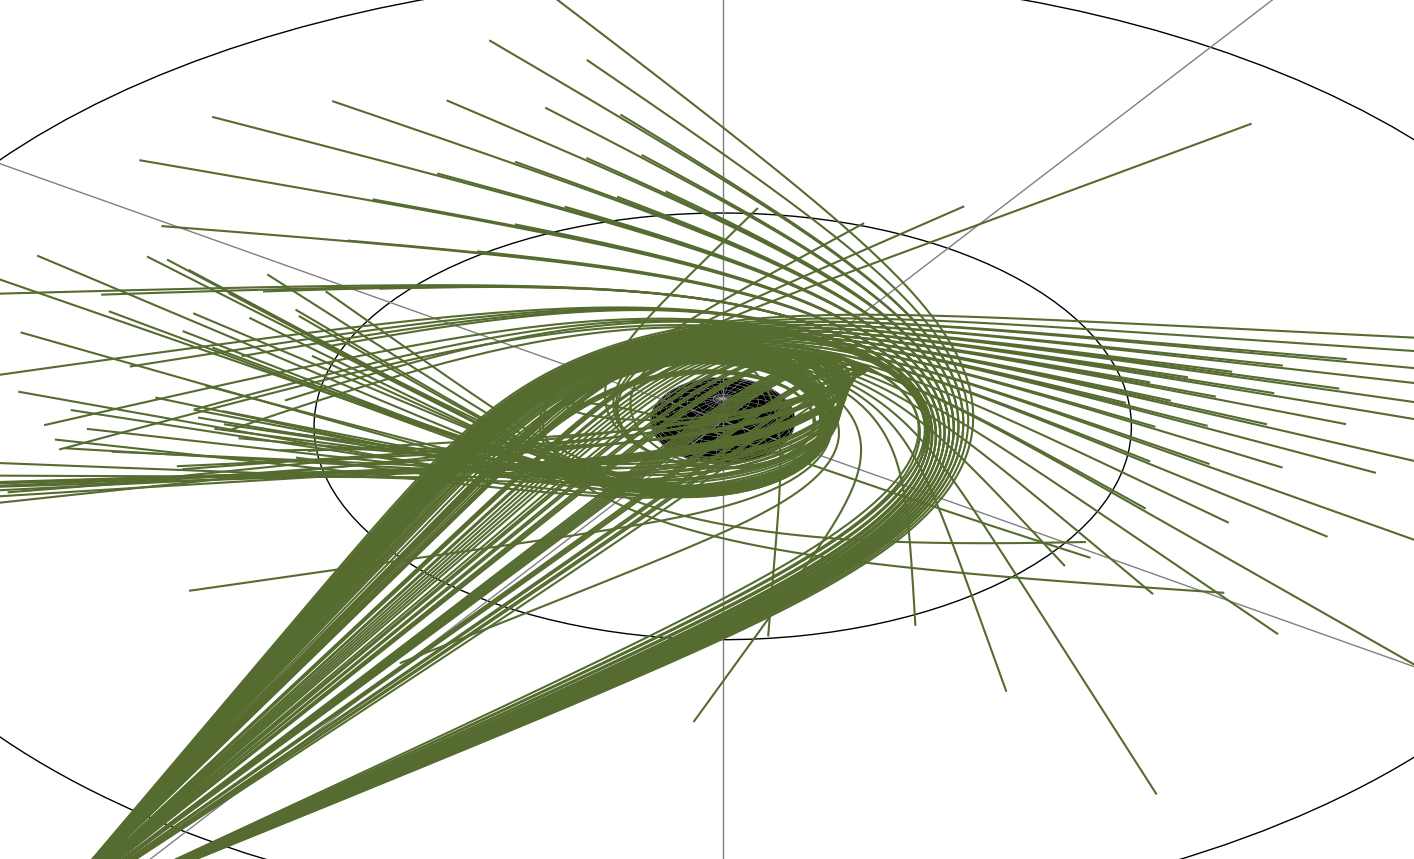
\includegraphics[width=.35\linewidth]{gfx/halo_entero}}}
	\caption[Disk geodesics study]{Disk geodesics study}\label{fig:diskgeodesicstudy}
\end{figure}

\subsubsection*{Infinite Images}

The shadow and the \ac{ISCO} are very close, so near the \ac{ISCO}, the particles turn around the black holes a great number of times. The previous study showed only the case where the particles make one full turn, but between that inner halo and the shadow there are an infinite number of halos, as for every turn completed by a geodesic, an image of the halo is generated near the black hole. A study on the shadow formation and geodesics near the \ac{ISCO} was also done. \autoref{fig:virtualshadow} depicts parallel geodesics that fall in the black hole. As we saw, the shadow seen on the right part of the image is much greater than the actual diameter of the black hole's horizon. That way, the shadow is not the black hole's horizon but the diameter for which the contained geodesics fall inside it. We could study the \ac{ISCO} by studying geodesics that turn close to the horizon. \autoref{fig:isco} shows two examples of a set of geodesics on the equatorial plane that turn around the horizon once.

\begin{figure}[bth]
	\myfloatalign
	\subfloat[Horizon and shadow]
	{\label{fig:virtualshadow}
		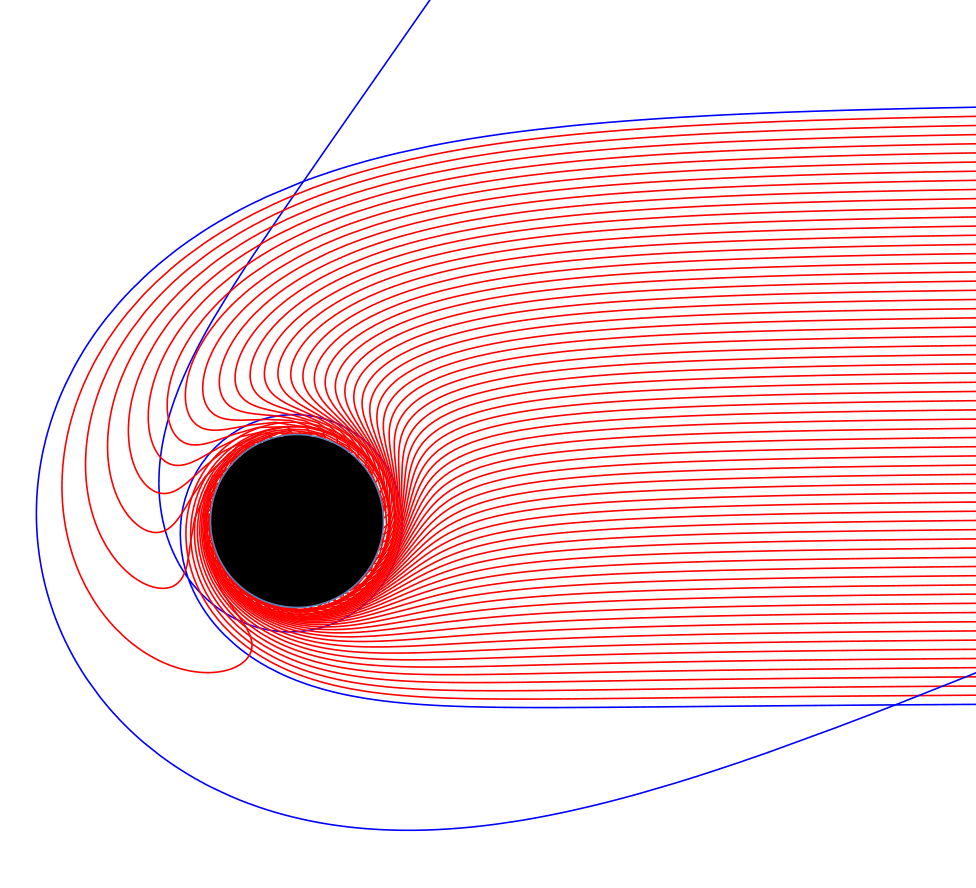
\includegraphics[width=.45\linewidth]{gfx/shadow}} \quad
	\subfloat[Loop around the shadow]
	{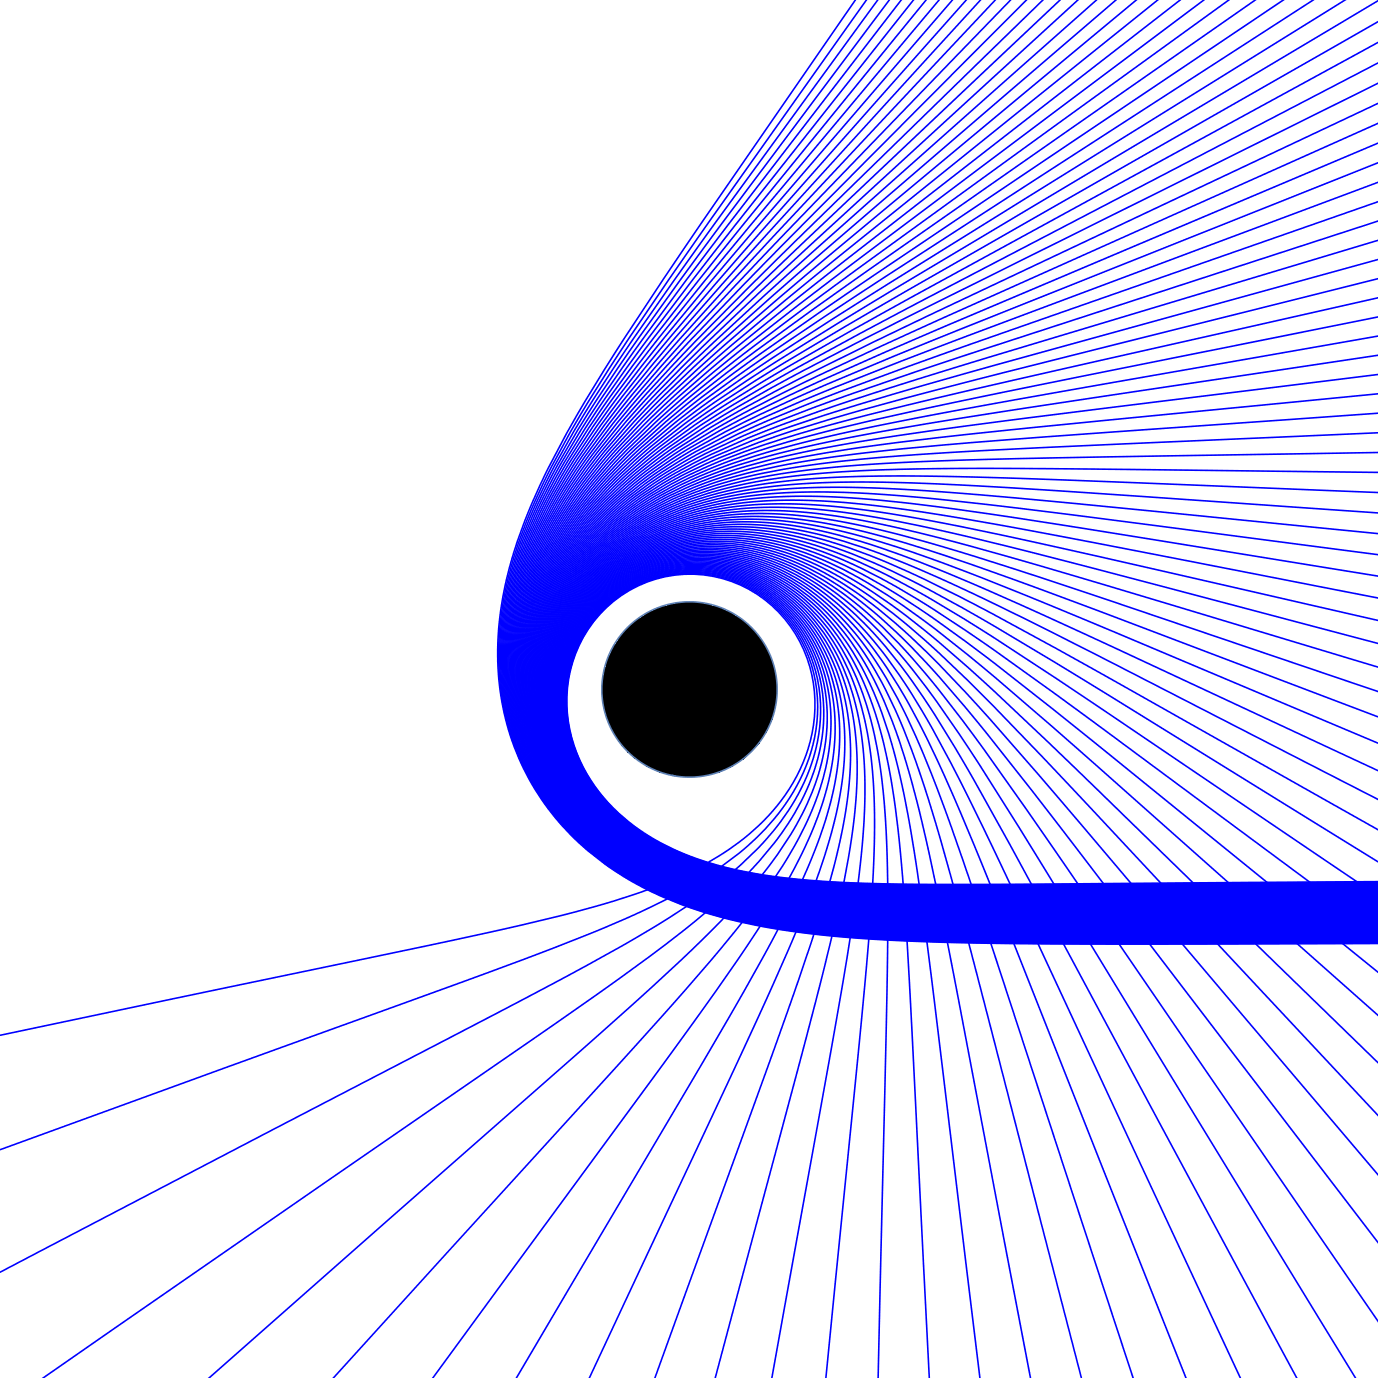
\includegraphics[width=.45\linewidth]{gfx/isco1}}
	\caption[Geodesics around the horizon]{Geodesics around the horizon.}
	\label{fig:isco}
\end{figure}